\documentclass[10pt,xcolor={dvipsnames}]{beamer}

\usetheme[progressbar=frametitle]{metropolis}
\usepackage{appendixnumberbeamer}

\usepackage{booktabs}
\usepackage[scale=2]{ccicons}

\usepackage{pgfplots}
\usepgfplotslibrary{dateplot}
\usepackage[utf8]{inputenc}

\usepackage{fancyvrb}


\usepackage{xspace}
\newcommand{\themename}{\textbf{\textsc{metropolis}}\xspace}
\newcommand\tab[1][1cm]{\hspace*{#1}}

\title{Flex}
\subtitle{Un generador de Scanners libre}
% \date{\today}
\date{}
\author{Jose Pablo Vargas Campos \newline 2013116365}
\institute{Instituto Tecnológico de Costa Rica\newline Compiladores e Intérpretes \newline Semestre 2017 }
% \titlegraphic{\hfill\includegraphics[height=1.5cm]{logo.pdf}}

\begin{document}

\maketitle

\begin{frame}{Table of contents}
  \setbeamertemplate{section in toc}[sections numbered]
  \tableofcontents[hideallsubsections]
\end{frame}

\section{Introducción}

\begin{frame}[fragile]{Introducción}


\begin{alertblock}{Introducción}
		Flex es una herramienta de análisis lexico desarrollada para la generación de Scanners de lenguajes. Su nombre significa "fast lexical analyzer generator". Es la alternativa gratis y open-source a la herramienta "lex". 
\end{alertblock}
    
\end{frame}
    
\begin{frame}[fragile]{Scanning}

	\begin{alertblock}{Scanning}
		El proceso de Scanning es el proceso por el cual se identifican los diferentes lexemas de un lenguaje. El proceso es tan simple como la ejecución de un Automata Deterministico Finito. Para la generación del Scanner con Flex se utilizan las expresiones regulares, conocidas como `RegEx', para indicarle a Flex que construya apartir de las expresiones regulares un DFA en C, el cual luego se usa para adquirir los diferentes lexemas del lenguaje que se planea `Scannear'.

	\end{alertblock}

\end{frame}


\section{Analisis Léxico}

\begin{frame}[fragile,allowframebreaks]{Histograma}
\begin{alertblock}{Histograma}
	A continuación se presenta un histograma el cual indica cuantas veces cada token fue encontrado cada 50 lineas, en el \textit{axis y} se puede ver la cantidad de ocurrencias mientras en el \textit{axis x} se muestra en cual rango de lineas de codigo sucedieron.
	\end{alertblock}
\end{frame}
\begin{frame}[fragile,allowframebreaks]{Histograma}
\begin{alertblock}{Histograma}
	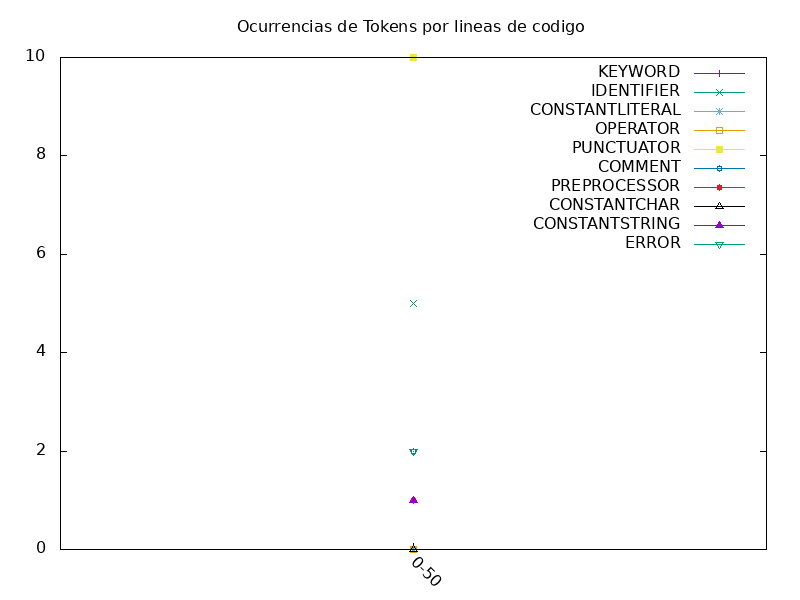
\includegraphics[scale=0.4]{histogram.png}
	\end{alertblock}
\end{frame}

\begin{frame}[fragile,allowframebreaks]{Analisis Léxico}
\begin{alertblock}{Codigo fuente}
	A continuación se presenta el codigo fuente con colores demostrando la división de Tokens.
	\end{alertblock}
\end{frame}
\begin{frame}[fragile,allowframebreaks]{Syntax Highlighting}~\color{Rhodamine}\begin{verbatim}/*
 *  linux/init/main.c
 *
 *  Copyright (C) 1991, 1992  Linus Torvalds
 *
 *  GK 2/5/95  -  Changed to support mounting root fs via NFS
 *  Added initrd & change_root: Werner Almesberger & Hans Lermen, Feb '96
 *  Moan early if gcc is old, avoiding bogus kernels - Paul Gortmaker, May '96
 *  Simplified starting of init:  Michael A. Griffith <grif@acm.org>
 */\end{verbatim}\leavevmode\newline\newline\color{Gray}\verb$#define DEBUG		/* Enable initcall_debug */$\newline\newline\color{Gray}\verb$#include <linux/types.h>$\newline\color{Gray}\verb$#include <linux/extable.h>$\newline\color{Gray}\verb$#include <linux/module.h>$\newline\color{Gray}\verb$#include <linux/proc_fs.h>$\newline\color{Gray}\verb$#include <linux/binfmts.h>$\newline\color{Gray}\verb$#include <linux/kernel.h>$\newline\color{Gray}\verb$#include <linux/syscalls.h>$\newline\color{Gray}\verb$#include <linux/stackprotector.h>$\newline\color{Gray}\verb$#include <linux/string.h>$\newline\color{Gray}\verb$#include <linux/ctype.h>$\newline\color{Gray}\verb$#include <linux/delay.h>$\newline\color{Gray}\verb$#include <linux/ioport.h>$\newline\color{Gray}\verb$#include <linux/init.h>$\newline\color{Gray}\verb$#include <linux/initrd.h>$\newline\color{Gray}\verb$#include <linux/bootmem.h>$\newline\color{Gray}\verb$#include <linux/acpi.h>$\newline\color{Gray}\verb$#include <linux/console.h>$\newline\color{Gray}\verb$#include <linux/nmi.h>$\newline\color{Gray}\verb$#include <linux/percpu.h>$\newline\color{Gray}\verb$#include <linux/kmod.h>$\newline\color{Gray}\verb$#include <linux/vmalloc.h>$\newline\color{Gray}\verb$#include <linux/kernel_stat.h>$\newline\color{Gray}\verb$#include <linux/start_kernel.h>$\newline\color{Gray}\verb$#include <linux/security.h>$\newline\color{Gray}\verb$#include <linux/smp.h>$\newline\color{Gray}\verb$#include <linux/profile.h>$\newline\color{Gray}\verb$#include <linux/rcupdate.h>$\newline\color{Gray}\verb$#include <linux/moduleparam.h>$\newline\color{Gray}\verb$#include <linux/kallsyms.h>$\newline\color{Gray}\verb$#include <linux/writeback.h>$\newline\color{Gray}\verb$#include <linux/cpu.h>$\newline\color{Gray}\verb$#include <linux/cpuset.h>$\newline\color{Gray}\verb$#include <linux/cgroup.h>$\newline\color{Gray}\verb$#include <linux/efi.h>$\newline\color{Gray}\verb$#include <linux/tick.h>$\newline\color{Gray}\verb$#include <linux/interrupt.h>$\newline\color{Gray}\verb$#include <linux/taskstats_kern.h>$\newline\color{Gray}\verb$#include <linux/delayacct.h>$\newline\color{Gray}\verb$#include <linux/unistd.h>$\newline\color{Gray}\verb$#include <linux/rmap.h>$\newline\color{Gray}\verb$#include <linux/mempolicy.h>$\newline\color{Gray}\verb$#include <linux/key.h>$\newline\color{Gray}\verb$#include <linux/buffer_head.h>$\newline\color{Gray}\verb$#include <linux/page_ext.h>$\newline\color{Gray}\verb$#include <linux/debug_locks.h>$\newline\color{Gray}\verb$#include <linux/debugobjects.h>$\newline\color{Gray}\verb$#include <linux/lockdep.h>$\newline\color{Gray}\verb$#include <linux/kmemleak.h>$\newline\color{Gray}\verb$#include <linux/pid_namespace.h>$\newline\color{Gray}\verb$#include <linux/device.h>$\newline\color{Gray}\verb$#include <linux/kthread.h>$\newline\color{Gray}\verb$#include <linux/sched.h>$\newline\color{Gray}\verb$#include <linux/sched/init.h>$\newline\color{Gray}\verb$#include <linux/signal.h>$\newline\color{Gray}\verb$#include <linux/idr.h>$\newline\color{Gray}\verb$#include <linux/kgdb.h>$\newline\color{Gray}\verb$#include <linux/ftrace.h>$\newline\color{Gray}\verb$#include <linux/async.h>$\newline\color{Gray}\verb$#include <linux/kmemcheck.h>$\newline\color{Gray}\verb$#include <linux/sfi.h>$\newline\color{Gray}\verb$#include <linux/shmem_fs.h>$\newline\color{Gray}\verb$#include <linux/slab.h>$\newline\color{Gray}\verb$#include <linux/perf_event.h>$\newline\color{Gray}\verb$#include <linux/ptrace.h>$\newline\color{Gray}\verb$#include <linux/blkdev.h>$\newline\color{Gray}\verb$#include <linux/elevator.h>$\newline\color{Gray}\verb$#include <linux/sched_clock.h>$\newline\color{Gray}\verb$#include <linux/sched/task.h>$\newline\color{Gray}\verb$#include <linux/sched/task_stack.h>$\newline\color{Gray}\verb$#include <linux/context_tracking.h>$\newline\color{Gray}\verb$#include <linux/random.h>$\newline\color{Gray}\verb$#include <linux/list.h>$\newline\color{Gray}\verb$#include <linux/integrity.h>$\newline\color{Gray}\verb$#include <linux/proc_ns.h>$\newline\color{Gray}\verb$#include <linux/io.h>$\newline\color{Gray}\verb$#include <linux/cache.h>$\newline\color{Gray}\verb$#include <linux/rodata_test.h>$\newline\newline\color{Gray}\verb$#include <asm/io.h>$\newline\color{Gray}\verb$#include <asm/bugs.h>$\newline\color{Gray}\verb$#include <asm/setup.h>$\newline\color{Gray}\verb$#include <asm/sections.h>$\newline\color{Gray}\verb$#include <asm/cacheflush.h>$\newline\newline\color{BurntOrange}\verb$static$ \color{BurntOrange}\verb$int$ \color{Aquamarine}\verb$kernel_init$\color{Fuchsia}\verb$($\color{BurntOrange}\verb$void$ \color{Goldenrod}\verb$*$\color{Fuchsia}\verb$)$\color{Fuchsia}\verb$;$\newline\newline\color{BurntOrange}\verb$extern$ \color{BurntOrange}\verb$void$ \color{Aquamarine}\verb$init_IRQ$\color{Fuchsia}\verb$($\color{BurntOrange}\verb$void$\color{Fuchsia}\verb$)$\color{Fuchsia}\verb$;$\newline\color{BurntOrange}\verb$extern$ \color{BurntOrange}\verb$void$ \color{Aquamarine}\verb$fork_init$\color{Fuchsia}\verb$($\color{BurntOrange}\verb$void$\color{Fuchsia}\verb$)$\color{Fuchsia}\verb$;$\newline\color{BurntOrange}\verb$extern$ \color{BurntOrange}\verb$void$ \color{Aquamarine}\verb$radix_tree_init$\color{Fuchsia}\verb$($\color{BurntOrange}\verb$void$\color{Fuchsia}\verb$)$\color{Fuchsia}\verb$;$\newline\newline\color{Rhodamine}\begin{verbatim}/*
 * Debug helper: via this flag we know that we are in 'early bootup code'
 * where only the boot processor is running with IRQ disabled.  This means
 * two things - IRQ must not be enabled before the flag is cleared and some
 * operations which are not allowed with IRQ disabled are allowed while the
 * flag is set.
 */\end{verbatim}\leavevmode\newline\color{Aquamarine}\verb$bool$ \color{Aquamarine}\verb$early_boot_irqs_disabled$ \color{Aquamarine}\verb$__read_mostly$\color{Fuchsia}\verb$;$\newline\newline\color{BurntOrange}\verb$enum$ \color{Aquamarine}\verb$system_states$ \color{Aquamarine}\verb$system_state$ \color{Aquamarine}\verb$__read_mostly$\color{Fuchsia}\verb$;$\newline\color{Aquamarine}\verb$EXPORT_SYMBOL$\color{Fuchsia}\verb$($\color{Aquamarine}\verb$system_state$\color{Fuchsia}\verb$)$\color{Fuchsia}\verb$;$\newline\newline\color{Rhodamine}\begin{verbatim}/*
 * Boot command-line arguments
 */\end{verbatim}\leavevmode\newline\color{Gray}\verb$#define MAX_INIT_ARGS CONFIG_INIT_ENV_ARG_LIMIT$\newline\color{Gray}\verb$#define MAX_INIT_ENVS CONFIG_INIT_ENV_ARG_LIMIT$\newline\newline\color{BurntOrange}\verb$extern$ \color{BurntOrange}\verb$void$ \color{Aquamarine}\verb$time_init$\color{Fuchsia}\verb$($\color{BurntOrange}\verb$void$\color{Fuchsia}\verb$)$\color{Fuchsia}\verb$;$\newline\color{Rhodamine}\begin{verbatim}/* Default late time init is NULL. archs can override this later. */\end{verbatim}\leavevmode\newline\color{BurntOrange}\verb$void$ \color{Fuchsia}\verb$($\color{Goldenrod}\verb$*$\color{Aquamarine}\verb$__initdata$ \color{Aquamarine}\verb$late_time_init$\color{Fuchsia}\verb$)$\color{Fuchsia}\verb$($\color{BurntOrange}\verb$void$\color{Fuchsia}\verb$)$\color{Fuchsia}\verb$;$\newline\newline\color{Rhodamine}\begin{verbatim}/* Untouched command line saved by arch-specific code. */\end{verbatim}\leavevmode\newline\color{BurntOrange}\verb$char$ \color{Aquamarine}\verb$__initdata$ \color{Aquamarine}\verb$boot_command_line$\color{Fuchsia}\verb$[$\color{Aquamarine}\verb$COMMAND_LINE_SIZE$\color{Fuchsia}\verb$]$\color{Fuchsia}\verb$;$\newline\color{Rhodamine}\begin{verbatim}/* Untouched saved command line (eg. for /proc) */\end{verbatim}\leavevmode\newline\color{BurntOrange}\verb$char$ \color{Goldenrod}\verb$*$\color{Aquamarine}\verb$saved_command_line$\color{Fuchsia}\verb$;$\newline\color{Rhodamine}\begin{verbatim}/* Command line for parameter parsing */\end{verbatim}\leavevmode\newline\color{BurntOrange}\verb$static$ \color{BurntOrange}\verb$char$ \color{Goldenrod}\verb$*$\color{Aquamarine}\verb$static_command_line$\color{Fuchsia}\verb$;$\newline\color{Rhodamine}\begin{verbatim}/* Command line for per-initcall parameter parsing */\end{verbatim}\leavevmode\newline\color{BurntOrange}\verb$static$ \color{BurntOrange}\verb$char$ \color{Goldenrod}\verb$*$\color{Aquamarine}\verb$initcall_command_line$\color{Fuchsia}\verb$;$\newline\newline\color{BurntOrange}\verb$static$ \color{BurntOrange}\verb$char$ \color{Goldenrod}\verb$*$\color{Aquamarine}\verb$execute_command$\color{Fuchsia}\verb$;$\newline\color{BurntOrange}\verb$static$ \color{BurntOrange}\verb$char$ \color{Goldenrod}\verb$*$\color{Aquamarine}\verb$ramdisk_execute_command$\color{Fuchsia}\verb$;$\newline\newline\color{Rhodamine}\begin{verbatim}/*
 * Used to generate warnings if static_key manipulation functions are used
 * before jump_label_init is called.
 */\end{verbatim}\leavevmode\newline\color{Aquamarine}\verb$bool$ \color{Aquamarine}\verb$static_key_initialized$ \color{Aquamarine}\verb$__read_mostly$\color{Fuchsia}\verb$;$\newline\color{Aquamarine}\verb$EXPORT_SYMBOL_GPL$\color{Fuchsia}\verb$($\color{Aquamarine}\verb$static_key_initialized$\color{Fuchsia}\verb$)$\color{Fuchsia}\verb$;$\newline\newline\color{Rhodamine}\begin{verbatim}/*
 * If set, this is an indication to the drivers that reset the underlying
 * device before going ahead with the initialization otherwise driver might
 * rely on the BIOS and skip the reset operation.
 *
 * This is useful if kernel is booting in an unreliable environment.
 * For ex. kdump situation where previous kernel has crashed, BIOS has been
 * skipped and devices will be in unknown state.
 */\end{verbatim}\leavevmode\newline\color{BurntOrange}\verb$unsigned$ \color{BurntOrange}\verb$int$ \color{Aquamarine}\verb$reset_devices$\color{Fuchsia}\verb$;$\newline\color{Aquamarine}\verb$EXPORT_SYMBOL$\color{Fuchsia}\verb$($\color{Aquamarine}\verb$reset_devices$\color{Fuchsia}\verb$)$\color{Fuchsia}\verb$;$\newline\newline\color{BurntOrange}\verb$static$ \color{BurntOrange}\verb$int$ \color{Aquamarine}\verb$__init$ \color{Aquamarine}\verb$set_reset_devices$\color{Fuchsia}\verb$($\color{BurntOrange}\verb$char$ \color{Goldenrod}\verb$*$\color{Aquamarine}\verb$str$\color{Fuchsia}\verb$)$\newline\color{Fuchsia}\verb${$\newline\tab\color{Aquamarine}\verb$reset_devices$ \color{Fuchsia}\verb$=$ \color{ForestGreen}\verb$1$\color{Fuchsia}\verb$;$\newline\tab\color{BurntOrange}\verb$return$ \color{ForestGreen}\verb$1$\color{Fuchsia}\verb$;$\newline\color{Fuchsia}\verb$}$\newline\newline\color{Aquamarine}\verb$__setup$\color{Fuchsia}\verb$($\color{Emerald}\verb$"reset_devices"$\color{Fuchsia}\verb$,$ \color{Aquamarine}\verb$set_reset_devices$\color{Fuchsia}\verb$)$\color{Fuchsia}\verb$;$\newline\newline\color{BurntOrange}\verb$static$ \color{BurntOrange}\verb$const$ \color{BurntOrange}\verb$char$ \color{Goldenrod}\verb$*$\color{Aquamarine}\verb$argv_init$\color{Fuchsia}\verb$[$\color{Aquamarine}\verb$MAX_INIT_ARGS$\color{ForestGreen}\verb$+2$\color{Fuchsia}\verb$]$ \color{Fuchsia}\verb$=$ \color{Fuchsia}\verb${$ \color{Emerald}\verb$"init"$\color{Fuchsia}\verb$,$ \color{Aquamarine}\verb$NULL$\color{Fuchsia}\verb$,$ \color{Fuchsia}\verb$}$\color{Fuchsia}\verb$;$\newline\color{BurntOrange}\verb$const$ \color{BurntOrange}\verb$char$ \color{Goldenrod}\verb$*$\color{Aquamarine}\verb$envp_init$\color{Fuchsia}\verb$[$\color{Aquamarine}\verb$MAX_INIT_ENVS$\color{ForestGreen}\verb$+2$\color{Fuchsia}\verb$]$ \color{Fuchsia}\verb$=$ \color{Fuchsia}\verb${$ \color{Emerald}\verb$"HOME=/"$\color{Fuchsia}\verb$,$ \color{Emerald}\verb$"TERM=linux"$\color{Fuchsia}\verb$,$ \color{Aquamarine}\verb$NULL$\color{Fuchsia}\verb$,$ \color{Fuchsia}\verb$}$\color{Fuchsia}\verb$;$\newline\color{BurntOrange}\verb$static$ \color{BurntOrange}\verb$const$ \color{BurntOrange}\verb$char$ \color{Goldenrod}\verb$*$\color{Aquamarine}\verb$panic_later$\color{Fuchsia}\verb$,$ \color{Goldenrod}\verb$*$\color{Aquamarine}\verb$panic_param$\color{Fuchsia}\verb$;$\newline\newline\color{BurntOrange}\verb$extern$ \color{BurntOrange}\verb$const$ \color{BurntOrange}\verb$struct$ \color{Aquamarine}\verb$obs_kernel_param$ \color{Aquamarine}\verb$__setup_start$\color{Fuchsia}\verb$[$\color{Fuchsia}\verb$]$\color{Fuchsia}\verb$,$ \color{Aquamarine}\verb$__setup_end$\color{Fuchsia}\verb$[$\color{Fuchsia}\verb$]$\color{Fuchsia}\verb$;$\newline\newline\color{BurntOrange}\verb$static$ \color{Aquamarine}\verb$bool$ \color{Aquamarine}\verb$__init$ \color{Aquamarine}\verb$obsolete_checksetup$\color{Fuchsia}\verb$($\color{BurntOrange}\verb$char$ \color{Goldenrod}\verb$*$\color{Aquamarine}\verb$line$\color{Fuchsia}\verb$)$\newline\color{Fuchsia}\verb${$\newline\tab\color{BurntOrange}\verb$const$ \color{BurntOrange}\verb$struct$ \color{Aquamarine}\verb$obs_kernel_param$ \color{Goldenrod}\verb$*$\color{Aquamarine}\verb$p$\color{Fuchsia}\verb$;$\newline\tab\color{Aquamarine}\verb$bool$ \color{Aquamarine}\verb$had_early_param$ \color{Fuchsia}\verb$=$ \color{Aquamarine}\verb$false$\color{Fuchsia}\verb$;$\newline\newline\tab\color{Aquamarine}\verb$p$ \color{Fuchsia}\verb$=$ \color{Aquamarine}\verb$__setup_start$\color{Fuchsia}\verb$;$\newline\tab\color{BurntOrange}\verb$do$ \color{Fuchsia}\verb${$\newline\tab\tab\color{BurntOrange}\verb$int$ \color{Aquamarine}\verb$n$ \color{Fuchsia}\verb$=$ \color{Aquamarine}\verb$strlen$\color{Fuchsia}\verb$($\color{Aquamarine}\verb$p$\color{Goldenrod}\verb$-$\color{Goldenrod}\verb$>$\color{Aquamarine}\verb$str$\color{Fuchsia}\verb$)$\color{Fuchsia}\verb$;$\newline\tab\tab\color{BurntOrange}\verb$if$ \color{Fuchsia}\verb$($\color{Aquamarine}\verb$parameqn$\color{Fuchsia}\verb$($\color{Aquamarine}\verb$line$\color{Fuchsia}\verb$,$ \color{Aquamarine}\verb$p$\color{Goldenrod}\verb$-$\color{Goldenrod}\verb$>$\color{Aquamarine}\verb$str$\color{Fuchsia}\verb$,$ \color{Aquamarine}\verb$n$\color{Fuchsia}\verb$)$\color{Fuchsia}\verb$)$ \color{Fuchsia}\verb${$\newline\tab\tab\tab\color{BurntOrange}\verb$if$ \color{Fuchsia}\verb$($\color{Aquamarine}\verb$p$\color{Goldenrod}\verb$-$\color{Goldenrod}\verb$>$\color{Aquamarine}\verb$early$\color{Fuchsia}\verb$)$ \color{Fuchsia}\verb${$\newline\tab\tab\tab\tab\color{Rhodamine}\begin{verbatim}/* Already done in parse_early_param?
				 * (Needs exact match on param part).
				 * Keep iterating, as we can have early
				 * params and __setups of same names 8( */\end{verbatim}\leavevmode\newline\tab\tab\tab\tab\color{BurntOrange}\verb$if$ \color{Fuchsia}\verb$($\color{Aquamarine}\verb$line$\color{Fuchsia}\verb$[$\color{Aquamarine}\verb$n$\color{Fuchsia}\verb$]$ \color{Goldenrod}\verb$==$ \color{GreenYellow}\verb$'\0'$ \color{Goldenrod}\verb$||$ \color{Aquamarine}\verb$line$\color{Fuchsia}\verb$[$\color{Aquamarine}\verb$n$\color{Fuchsia}\verb$]$ \color{Goldenrod}\verb$==$ \color{GreenYellow}\verb$'='$\color{Fuchsia}\verb$)$\newline\tab\tab\tab\tab\tab\color{Aquamarine}\verb$had_early_param$ \color{Fuchsia}\verb$=$ \color{Aquamarine}\verb$true$\color{Fuchsia}\verb$;$\newline\tab\tab\tab\color{Fuchsia}\verb$}$ \color{BurntOrange}\verb$else$ \color{BurntOrange}\verb$if$ \color{Fuchsia}\verb$($\color{Goldenrod}\verb$!$\color{Aquamarine}\verb$p$\color{Goldenrod}\verb$-$\color{Goldenrod}\verb$>$\color{Aquamarine}\verb$setup_func$\color{Fuchsia}\verb$)$ \color{Fuchsia}\verb${$\newline\tab\tab\tab\tab\color{Aquamarine}\verb$pr_warn$\color{Fuchsia}\verb$($\color{Emerald}\verb$"Parameter %s is obsolete, ignored\n"$\color{Fuchsia}\verb$,$\newline\tab\tab\tab\tab\tab\color{Aquamarine}\verb$p$\color{Goldenrod}\verb$-$\color{Goldenrod}\verb$>$\color{Aquamarine}\verb$str$\color{Fuchsia}\verb$)$\color{Fuchsia}\verb$;$\newline\tab\tab\tab\tab\color{BurntOrange}\verb$return$ \color{Aquamarine}\verb$true$\color{Fuchsia}\verb$;$\newline\tab\tab\tab\color{Fuchsia}\verb$}$ \color{BurntOrange}\verb$else$ \color{BurntOrange}\verb$if$ \color{Fuchsia}\verb$($\color{Aquamarine}\verb$p$\color{Goldenrod}\verb$-$\color{Goldenrod}\verb$>$\color{Aquamarine}\verb$setup_func$\color{Fuchsia}\verb$($\color{Aquamarine}\verb$line$ \color{Goldenrod}\verb$+$ \color{Aquamarine}\verb$n$\color{Fuchsia}\verb$)$\color{Fuchsia}\verb$)$\newline\tab\tab\tab\tab\color{BurntOrange}\verb$return$ \color{Aquamarine}\verb$true$\color{Fuchsia}\verb$;$\newline\tab\tab\color{Fuchsia}\verb$}$\newline\tab\tab\color{Aquamarine}\verb$p$\color{Goldenrod}\verb$++$\color{Fuchsia}\verb$;$\newline\tab\color{Fuchsia}\verb$}$ \color{BurntOrange}\verb$while$ \color{Fuchsia}\verb$($\color{Aquamarine}\verb$p$ \color{Goldenrod}\verb$<$ \color{Aquamarine}\verb$__setup_end$\color{Fuchsia}\verb$)$\color{Fuchsia}\verb$;$\newline\newline\tab\color{BurntOrange}\verb$return$ \color{Aquamarine}\verb$had_early_param$\color{Fuchsia}\verb$;$\newline\color{Fuchsia}\verb$}$\newline\newline\color{Rhodamine}\begin{verbatim}/*
 * This should be approx 2 Bo*oMips to start (note initial shift), and will
 * still work even if initially too large, it will just take slightly longer
 */\end{verbatim}\leavevmode\newline\color{BurntOrange}\verb$unsigned$ \color{BurntOrange}\verb$long$ \color{Aquamarine}\verb$loops_per_jiffy$ \color{Fuchsia}\verb$=$ \color{Fuchsia}\verb$($\color{ForestGreen}\verb$1$\color{Goldenrod}\verb$<<$\color{ForestGreen}\verb$12$\color{Fuchsia}\verb$)$\color{Fuchsia}\verb$;$\newline\color{Aquamarine}\verb$EXPORT_SYMBOL$\color{Fuchsia}\verb$($\color{Aquamarine}\verb$loops_per_jiffy$\color{Fuchsia}\verb$)$\color{Fuchsia}\verb$;$\newline\newline\color{BurntOrange}\verb$static$ \color{BurntOrange}\verb$int$ \color{Aquamarine}\verb$__init$ \color{Aquamarine}\verb$debug_kernel$\color{Fuchsia}\verb$($\color{BurntOrange}\verb$char$ \color{Goldenrod}\verb$*$\color{Aquamarine}\verb$str$\color{Fuchsia}\verb$)$\newline\color{Fuchsia}\verb${$\newline\tab\color{Aquamarine}\verb$console_loglevel$ \color{Fuchsia}\verb$=$ \color{Aquamarine}\verb$CONSOLE_LOGLEVEL_DEBUG$\color{Fuchsia}\verb$;$\newline\tab\color{BurntOrange}\verb$return$ \color{ForestGreen}\verb$0$\color{Fuchsia}\verb$;$\newline\color{Fuchsia}\verb$}$\newline\newline\color{BurntOrange}\verb$static$ \color{BurntOrange}\verb$int$ \color{Aquamarine}\verb$__init$ \color{Aquamarine}\verb$quiet_kernel$\color{Fuchsia}\verb$($\color{BurntOrange}\verb$char$ \color{Goldenrod}\verb$*$\color{Aquamarine}\verb$str$\color{Fuchsia}\verb$)$\newline\color{Fuchsia}\verb${$\newline\tab\color{Aquamarine}\verb$console_loglevel$ \color{Fuchsia}\verb$=$ \color{Aquamarine}\verb$CONSOLE_LOGLEVEL_QUIET$\color{Fuchsia}\verb$;$\newline\tab\color{BurntOrange}\verb$return$ \color{ForestGreen}\verb$0$\color{Fuchsia}\verb$;$\newline\color{Fuchsia}\verb$}$\newline\newline\color{Aquamarine}\verb$early_param$\color{Fuchsia}\verb$($\color{Emerald}\verb$"debug"$\color{Fuchsia}\verb$,$ \color{Aquamarine}\verb$debug_kernel$\color{Fuchsia}\verb$)$\color{Fuchsia}\verb$;$\newline\color{Aquamarine}\verb$early_param$\color{Fuchsia}\verb$($\color{Emerald}\verb$"quiet"$\color{Fuchsia}\verb$,$ \color{Aquamarine}\verb$quiet_kernel$\color{Fuchsia}\verb$)$\color{Fuchsia}\verb$;$\newline\newline\color{BurntOrange}\verb$static$ \color{BurntOrange}\verb$int$ \color{Aquamarine}\verb$__init$ \color{Aquamarine}\verb$loglevel$\color{Fuchsia}\verb$($\color{BurntOrange}\verb$char$ \color{Goldenrod}\verb$*$\color{Aquamarine}\verb$str$\color{Fuchsia}\verb$)$\newline\color{Fuchsia}\verb${$\newline\tab\color{BurntOrange}\verb$int$ \color{Aquamarine}\verb$newlevel$\color{Fuchsia}\verb$;$\newline\newline\tab\color{Rhodamine}\begin{verbatim}/*
	 * Only update loglevel value when a correct setting was passed,
	 * to prevent blind crashes (when loglevel being set to 0) that
	 * are quite hard to debug
	 */\end{verbatim}\leavevmode\newline\tab\color{BurntOrange}\verb$if$ \color{Fuchsia}\verb$($\color{Aquamarine}\verb$get_option$\color{Fuchsia}\verb$($\color{Goldenrod}\verb$&$\color{Aquamarine}\verb$str$\color{Fuchsia}\verb$,$ \color{Goldenrod}\verb$&$\color{Aquamarine}\verb$newlevel$\color{Fuchsia}\verb$)$\color{Fuchsia}\verb$)$ \color{Fuchsia}\verb${$\newline\tab\tab\color{Aquamarine}\verb$console_loglevel$ \color{Fuchsia}\verb$=$ \color{Aquamarine}\verb$newlevel$\color{Fuchsia}\verb$;$\newline\tab\tab\color{BurntOrange}\verb$return$ \color{ForestGreen}\verb$0$\color{Fuchsia}\verb$;$\newline\tab\color{Fuchsia}\verb$}$\newline\newline\tab\color{BurntOrange}\verb$return$ \color{Goldenrod}\verb$-$\color{Aquamarine}\verb$EINVAL$\color{Fuchsia}\verb$;$\newline\color{Fuchsia}\verb$}$\newline\newline\color{Aquamarine}\verb$early_param$\color{Fuchsia}\verb$($\color{Emerald}\verb$"loglevel"$\color{Fuchsia}\verb$,$ \color{Aquamarine}\verb$loglevel$\color{Fuchsia}\verb$)$\color{Fuchsia}\verb$;$\newline\newline\color{Rhodamine}\begin{verbatim}/* Change NUL term back to "=", to make "param" the whole string. */\end{verbatim}\leavevmode\newline\color{BurntOrange}\verb$static$ \color{BurntOrange}\verb$int$ \color{Aquamarine}\verb$__init$ \color{Aquamarine}\verb$repair_env_string$\color{Fuchsia}\verb$($\color{BurntOrange}\verb$char$ \color{Goldenrod}\verb$*$\color{Aquamarine}\verb$param$\color{Fuchsia}\verb$,$ \color{BurntOrange}\verb$char$ \color{Goldenrod}\verb$*$\color{Aquamarine}\verb$val$\color{Fuchsia}\verb$,$\newline\tab\tab\tab\tab    \color{BurntOrange}\verb$const$ \color{BurntOrange}\verb$char$ \color{Goldenrod}\verb$*$\color{Aquamarine}\verb$unused$\color{Fuchsia}\verb$,$ \color{BurntOrange}\verb$void$ \color{Goldenrod}\verb$*$\color{Aquamarine}\verb$arg$\color{Fuchsia}\verb$)$\newline\color{Fuchsia}\verb${$\newline\tab\color{BurntOrange}\verb$if$ \color{Fuchsia}\verb$($\color{Aquamarine}\verb$val$\color{Fuchsia}\verb$)$ \color{Fuchsia}\verb${$\newline\tab\tab\color{Rhodamine}\begin{verbatim}/* param=val or param="val"? */\end{verbatim}\leavevmode\newline\tab\tab\color{BurntOrange}\verb$if$ \color{Fuchsia}\verb$($\color{Aquamarine}\verb$val$ \color{Goldenrod}\verb$==$ \color{Aquamarine}\verb$param$\color{Goldenrod}\verb$+$\color{Aquamarine}\verb$strlen$\color{Fuchsia}\verb$($\color{Aquamarine}\verb$param$\color{Fuchsia}\verb$)$\color{ForestGreen}\verb$+1$\color{Fuchsia}\verb$)$\newline\tab\tab\tab\color{Aquamarine}\verb$val$\color{Fuchsia}\verb$[$\color{ForestGreen}\verb$-1$\color{Fuchsia}\verb$]$ \color{Fuchsia}\verb$=$ \color{GreenYellow}\verb$'='$\color{Fuchsia}\verb$;$\newline\tab\tab\color{BurntOrange}\verb$else$ \color{BurntOrange}\verb$if$ \color{Fuchsia}\verb$($\color{Aquamarine}\verb$val$ \color{Goldenrod}\verb$==$ \color{Aquamarine}\verb$param$\color{Goldenrod}\verb$+$\color{Aquamarine}\verb$strlen$\color{Fuchsia}\verb$($\color{Aquamarine}\verb$param$\color{Fuchsia}\verb$)$\color{ForestGreen}\verb$+2$\color{Fuchsia}\verb$)$ \color{Fuchsia}\verb${$\newline\tab\tab\tab\color{Aquamarine}\verb$val$\color{Fuchsia}\verb$[$\color{ForestGreen}\verb$-2$\color{Fuchsia}\verb$]$ \color{Fuchsia}\verb$=$ \color{GreenYellow}\verb$'='$\color{Fuchsia}\verb$;$
\end{frame}
\begin{frame}[fragile,allowframebreaks]{Syntax Highlighting}~\newline\tab\tab\tab\color{Aquamarine}\verb$memmove$\color{Fuchsia}\verb$($\color{Aquamarine}\verb$val$\color{ForestGreen}\verb$-1$\color{Fuchsia}\verb$,$ \color{Aquamarine}\verb$val$\color{Fuchsia}\verb$,$ \color{Aquamarine}\verb$strlen$\color{Fuchsia}\verb$($\color{Aquamarine}\verb$val$\color{Fuchsia}\verb$)$\color{ForestGreen}\verb$+1$\color{Fuchsia}\verb$)$\color{Fuchsia}\verb$;$\newline\tab\tab\tab\color{Aquamarine}\verb$val$\color{Goldenrod}\verb$--$\color{Fuchsia}\verb$;$\newline\tab\tab\color{Fuchsia}\verb$}$ \color{BurntOrange}\verb$else$\newline\tab\tab\tab\color{Aquamarine}\verb$BUG$\color{Fuchsia}\verb$($\color{Fuchsia}\verb$)$\color{Fuchsia}\verb$;$\newline\tab\color{Fuchsia}\verb$}$\newline\tab\color{BurntOrange}\verb$return$ \color{ForestGreen}\verb$0$\color{Fuchsia}\verb$;$\newline\color{Fuchsia}\verb$}$\newline\newline\color{Rhodamine}\begin{verbatim}/* Anything after -- gets handed straight to init. */\end{verbatim}\leavevmode\newline\color{BurntOrange}\verb$static$ \color{BurntOrange}\verb$int$ \color{Aquamarine}\verb$__init$ \color{Aquamarine}\verb$set_init_arg$\color{Fuchsia}\verb$($\color{BurntOrange}\verb$char$ \color{Goldenrod}\verb$*$\color{Aquamarine}\verb$param$\color{Fuchsia}\verb$,$ \color{BurntOrange}\verb$char$ \color{Goldenrod}\verb$*$\color{Aquamarine}\verb$val$\color{Fuchsia}\verb$,$\newline\tab\tab\tab       \color{BurntOrange}\verb$const$ \color{BurntOrange}\verb$char$ \color{Goldenrod}\verb$*$\color{Aquamarine}\verb$unused$\color{Fuchsia}\verb$,$ \color{BurntOrange}\verb$void$ \color{Goldenrod}\verb$*$\color{Aquamarine}\verb$arg$\color{Fuchsia}\verb$)$\newline\color{Fuchsia}\verb${$\newline\tab\color{BurntOrange}\verb$unsigned$ \color{BurntOrange}\verb$int$ \color{Aquamarine}\verb$i$\color{Fuchsia}\verb$;$\newline\newline\tab\color{BurntOrange}\verb$if$ \color{Fuchsia}\verb$($\color{Aquamarine}\verb$panic_later$\color{Fuchsia}\verb$)$\newline\tab\tab\color{BurntOrange}\verb$return$ \color{ForestGreen}\verb$0$\color{Fuchsia}\verb$;$\newline\newline\tab\color{Aquamarine}\verb$repair_env_string$\color{Fuchsia}\verb$($\color{Aquamarine}\verb$param$\color{Fuchsia}\verb$,$ \color{Aquamarine}\verb$val$\color{Fuchsia}\verb$,$ \color{Aquamarine}\verb$unused$\color{Fuchsia}\verb$,$ \color{Aquamarine}\verb$NULL$\color{Fuchsia}\verb$)$\color{Fuchsia}\verb$;$\newline\newline\tab\color{BurntOrange}\verb$for$ \color{Fuchsia}\verb$($\color{Aquamarine}\verb$i$ \color{Fuchsia}\verb$=$ \color{ForestGreen}\verb$0$\color{Fuchsia}\verb$;$ \color{Aquamarine}\verb$argv_init$\color{Fuchsia}\verb$[$\color{Aquamarine}\verb$i$\color{Fuchsia}\verb$]$\color{Fuchsia}\verb$;$ \color{Aquamarine}\verb$i$\color{Goldenrod}\verb$++$\color{Fuchsia}\verb$)$ \color{Fuchsia}\verb${$\newline\tab\tab\color{BurntOrange}\verb$if$ \color{Fuchsia}\verb$($\color{Aquamarine}\verb$i$ \color{Goldenrod}\verb$==$ \color{Aquamarine}\verb$MAX_INIT_ARGS$\color{Fuchsia}\verb$)$ \color{Fuchsia}\verb${$\newline\tab\tab\tab\color{Aquamarine}\verb$panic_later$ \color{Fuchsia}\verb$=$ \color{Emerald}\verb$"init"$\color{Fuchsia}\verb$;$\newline\tab\tab\tab\color{Aquamarine}\verb$panic_param$ \color{Fuchsia}\verb$=$ \color{Aquamarine}\verb$param$\color{Fuchsia}\verb$;$\newline\tab\tab\tab\color{BurntOrange}\verb$return$ \color{ForestGreen}\verb$0$\color{Fuchsia}\verb$;$\newline\tab\tab\color{Fuchsia}\verb$}$\newline\tab\color{Fuchsia}\verb$}$\newline\tab\color{Aquamarine}\verb$argv_init$\color{Fuchsia}\verb$[$\color{Aquamarine}\verb$i$\color{Fuchsia}\verb$]$ \color{Fuchsia}\verb$=$ \color{Aquamarine}\verb$param$\color{Fuchsia}\verb$;$\newline\tab\color{BurntOrange}\verb$return$ \color{ForestGreen}\verb$0$\color{Fuchsia}\verb$;$\newline\color{Fuchsia}\verb$}$\newline\newline\color{Rhodamine}\begin{verbatim}/*
 * Unknown boot options get handed to init, unless they look like
 * unused parameters (modprobe will find them in /proc/cmdline).
 */\end{verbatim}\leavevmode\newline\color{BurntOrange}\verb$static$ \color{BurntOrange}\verb$int$ \color{Aquamarine}\verb$__init$ \color{Aquamarine}\verb$unknown_bootoption$\color{Fuchsia}\verb$($\color{BurntOrange}\verb$char$ \color{Goldenrod}\verb$*$\color{Aquamarine}\verb$param$\color{Fuchsia}\verb$,$ \color{BurntOrange}\verb$char$ \color{Goldenrod}\verb$*$\color{Aquamarine}\verb$val$\color{Fuchsia}\verb$,$\newline\tab\tab\tab\tab     \color{BurntOrange}\verb$const$ \color{BurntOrange}\verb$char$ \color{Goldenrod}\verb$*$\color{Aquamarine}\verb$unused$\color{Fuchsia}\verb$,$ \color{BurntOrange}\verb$void$ \color{Goldenrod}\verb$*$\color{Aquamarine}\verb$arg$\color{Fuchsia}\verb$)$\newline\color{Fuchsia}\verb${$\newline\tab\color{Aquamarine}\verb$repair_env_string$\color{Fuchsia}\verb$($\color{Aquamarine}\verb$param$\color{Fuchsia}\verb$,$ \color{Aquamarine}\verb$val$\color{Fuchsia}\verb$,$ \color{Aquamarine}\verb$unused$\color{Fuchsia}\verb$,$ \color{Aquamarine}\verb$NULL$\color{Fuchsia}\verb$)$\color{Fuchsia}\verb$;$\newline\newline\tab\color{Rhodamine}\begin{verbatim}/* Handle obsolete-style parameters */\end{verbatim}\leavevmode\newline\tab\color{BurntOrange}\verb$if$ \color{Fuchsia}\verb$($\color{Aquamarine}\verb$obsolete_checksetup$\color{Fuchsia}\verb$($\color{Aquamarine}\verb$param$\color{Fuchsia}\verb$)$\color{Fuchsia}\verb$)$\newline\tab\tab\color{BurntOrange}\verb$return$ \color{ForestGreen}\verb$0$\color{Fuchsia}\verb$;$\newline\newline\tab\color{Rhodamine}\begin{verbatim}/* Unused module parameter. */\end{verbatim}\leavevmode\newline\tab\color{BurntOrange}\verb$if$ \color{Fuchsia}\verb$($\color{Aquamarine}\verb$strchr$\color{Fuchsia}\verb$($\color{Aquamarine}\verb$param$\color{Fuchsia}\verb$,$ \color{GreenYellow}\verb$'.'$\color{Fuchsia}\verb$)$ \color{Goldenrod}\verb$&&$ \color{Fuchsia}\verb$($\color{Goldenrod}\verb$!$\color{Aquamarine}\verb$val$ \color{Goldenrod}\verb$||$ \color{Aquamarine}\verb$strchr$\color{Fuchsia}\verb$($\color{Aquamarine}\verb$param$\color{Fuchsia}\verb$,$ \color{GreenYellow}\verb$'.'$\color{Fuchsia}\verb$)$ \color{Goldenrod}\verb$<$ \color{Aquamarine}\verb$val$\color{Fuchsia}\verb$)$\color{Fuchsia}\verb$)$\newline\tab\tab\color{BurntOrange}\verb$return$ \color{ForestGreen}\verb$0$\color{Fuchsia}\verb$;$\newline\newline\tab\color{BurntOrange}\verb$if$ \color{Fuchsia}\verb$($\color{Aquamarine}\verb$panic_later$\color{Fuchsia}\verb$)$\newline\tab\tab\color{BurntOrange}\verb$return$ \color{ForestGreen}\verb$0$\color{Fuchsia}\verb$;$\newline\newline\tab\color{BurntOrange}\verb$if$ \color{Fuchsia}\verb$($\color{Aquamarine}\verb$val$\color{Fuchsia}\verb$)$ \color{Fuchsia}\verb${$\newline\tab\tab\color{Rhodamine}\begin{verbatim}/* Environment option */\end{verbatim}\leavevmode\newline\tab\tab\color{BurntOrange}\verb$unsigned$ \color{BurntOrange}\verb$int$ \color{Aquamarine}\verb$i$\color{Fuchsia}\verb$;$\newline\tab\tab\color{BurntOrange}\verb$for$ \color{Fuchsia}\verb$($\color{Aquamarine}\verb$i$ \color{Fuchsia}\verb$=$ \color{ForestGreen}\verb$0$\color{Fuchsia}\verb$;$ \color{Aquamarine}\verb$envp_init$\color{Fuchsia}\verb$[$\color{Aquamarine}\verb$i$\color{Fuchsia}\verb$]$\color{Fuchsia}\verb$;$ \color{Aquamarine}\verb$i$\color{Goldenrod}\verb$++$\color{Fuchsia}\verb$)$ \color{Fuchsia}\verb${$\newline\tab\tab\tab\color{BurntOrange}\verb$if$ \color{Fuchsia}\verb$($\color{Aquamarine}\verb$i$ \color{Goldenrod}\verb$==$ \color{Aquamarine}\verb$MAX_INIT_ENVS$\color{Fuchsia}\verb$)$ \color{Fuchsia}\verb${$\newline\tab\tab\tab\tab\color{Aquamarine}\verb$panic_later$ \color{Fuchsia}\verb$=$ \color{Emerald}\verb$"env"$\color{Fuchsia}\verb$;$\newline\tab\tab\tab\tab\color{Aquamarine}\verb$panic_param$ \color{Fuchsia}\verb$=$ \color{Aquamarine}\verb$param$\color{Fuchsia}\verb$;$\newline\tab\tab\tab\color{Fuchsia}\verb$}$\newline\tab\tab\tab\color{BurntOrange}\verb$if$ \color{Fuchsia}\verb$($\color{Goldenrod}\verb$!$\color{Aquamarine}\verb$strncmp$\color{Fuchsia}\verb$($\color{Aquamarine}\verb$param$\color{Fuchsia}\verb$,$ \color{Aquamarine}\verb$envp_init$\color{Fuchsia}\verb$[$\color{Aquamarine}\verb$i$\color{Fuchsia}\verb$]$\color{Fuchsia}\verb$,$ \color{Aquamarine}\verb$val$ \color{Goldenrod}\verb$-$ \color{Aquamarine}\verb$param$\color{Fuchsia}\verb$)$\color{Fuchsia}\verb$)$\newline\tab\tab\tab\tab\color{BurntOrange}\verb$break$\color{Fuchsia}\verb$;$\newline\tab\tab\color{Fuchsia}\verb$}$\newline\tab\tab\color{Aquamarine}\verb$envp_init$\color{Fuchsia}\verb$[$\color{Aquamarine}\verb$i$\color{Fuchsia}\verb$]$ \color{Fuchsia}\verb$=$ \color{Aquamarine}\verb$param$\color{Fuchsia}\verb$;$\newline\tab\color{Fuchsia}\verb$}$ \color{BurntOrange}\verb$else$ \color{Fuchsia}\verb${$\newline\tab\tab\color{Rhodamine}\begin{verbatim}/* Command line option */\end{verbatim}\leavevmode\newline\tab\tab\color{BurntOrange}\verb$unsigned$ \color{BurntOrange}\verb$int$ \color{Aquamarine}\verb$i$\color{Fuchsia}\verb$;$\newline\tab\tab\color{BurntOrange}\verb$for$ \color{Fuchsia}\verb$($\color{Aquamarine}\verb$i$ \color{Fuchsia}\verb$=$ \color{ForestGreen}\verb$0$\color{Fuchsia}\verb$;$ \color{Aquamarine}\verb$argv_init$\color{Fuchsia}\verb$[$\color{Aquamarine}\verb$i$\color{Fuchsia}\verb$]$\color{Fuchsia}\verb$;$ \color{Aquamarine}\verb$i$\color{Goldenrod}\verb$++$\color{Fuchsia}\verb$)$ \color{Fuchsia}\verb${$\newline\tab\tab\tab\color{BurntOrange}\verb$if$ \color{Fuchsia}\verb$($\color{Aquamarine}\verb$i$ \color{Goldenrod}\verb$==$ \color{Aquamarine}\verb$MAX_INIT_ARGS$\color{Fuchsia}\verb$)$ \color{Fuchsia}\verb${$\newline\tab\tab\tab\tab\color{Aquamarine}\verb$panic_later$ \color{Fuchsia}\verb$=$ \color{Emerald}\verb$"init"$\color{Fuchsia}\verb$;$\newline\tab\tab\tab\tab\color{Aquamarine}\verb$panic_param$ \color{Fuchsia}\verb$=$ \color{Aquamarine}\verb$param$\color{Fuchsia}\verb$;$\newline\tab\tab\tab\color{Fuchsia}\verb$}$\newline\tab\tab\color{Fuchsia}\verb$}$\newline\tab\tab\color{Aquamarine}\verb$argv_init$\color{Fuchsia}\verb$[$\color{Aquamarine}\verb$i$\color{Fuchsia}\verb$]$ \color{Fuchsia}\verb$=$ \color{Aquamarine}\verb$param$\color{Fuchsia}\verb$;$\newline\tab\color{Fuchsia}\verb$}$\newline\tab\color{BurntOrange}\verb$return$ \color{ForestGreen}\verb$0$\color{Fuchsia}\verb$;$\newline\color{Fuchsia}\verb$}$\newline\newline\color{BurntOrange}\verb$static$ \color{BurntOrange}\verb$int$ \color{Aquamarine}\verb$__init$ \color{Aquamarine}\verb$init_setup$\color{Fuchsia}\verb$($\color{BurntOrange}\verb$char$ \color{Goldenrod}\verb$*$\color{Aquamarine}\verb$str$\color{Fuchsia}\verb$)$\newline\color{Fuchsia}\verb${$\newline\tab\color{BurntOrange}\verb$unsigned$ \color{BurntOrange}\verb$int$ \color{Aquamarine}\verb$i$\color{Fuchsia}\verb$;$\newline\newline\tab\color{Aquamarine}\verb$execute_command$ \color{Fuchsia}\verb$=$ \color{Aquamarine}\verb$str$\color{Fuchsia}\verb$;$\newline\tab\color{Rhodamine}\begin{verbatim}/*
	 * In case LILO is going to boot us with default command line,
	 * it prepends "auto" before the whole cmdline which makes
	 * the shell think it should execute a script with such name.
	 * So we ignore all arguments entered _before_ init=... [MJ]
	 */\end{verbatim}\leavevmode\newline\tab\color{BurntOrange}\verb$for$ \color{Fuchsia}\verb$($\color{Aquamarine}\verb$i$ \color{Fuchsia}\verb$=$ \color{ForestGreen}\verb$1$\color{Fuchsia}\verb$;$ \color{Aquamarine}\verb$i$ \color{Goldenrod}\verb$<$ \color{Aquamarine}\verb$MAX_INIT_ARGS$\color{Fuchsia}\verb$;$ \color{Aquamarine}\verb$i$\color{Goldenrod}\verb$++$\color{Fuchsia}\verb$)$\newline\tab\tab\color{Aquamarine}\verb$argv_init$\color{Fuchsia}\verb$[$\color{Aquamarine}\verb$i$\color{Fuchsia}\verb$]$ \color{Fuchsia}\verb$=$ \color{Aquamarine}\verb$NULL$\color{Fuchsia}\verb$;$\newline\tab\color{BurntOrange}\verb$return$ \color{ForestGreen}\verb$1$\color{Fuchsia}\verb$;$\newline\color{Fuchsia}\verb$}$\newline\color{Aquamarine}\verb$__setup$\color{Fuchsia}\verb$($\color{Emerald}\verb$"init="$\color{Fuchsia}\verb$,$ \color{Aquamarine}\verb$init_setup$\color{Fuchsia}\verb$)$\color{Fuchsia}\verb$;$\newline\newline\color{BurntOrange}\verb$static$ \color{BurntOrange}\verb$int$ \color{Aquamarine}\verb$__init$ \color{Aquamarine}\verb$rdinit_setup$\color{Fuchsia}\verb$($\color{BurntOrange}\verb$char$ \color{Goldenrod}\verb$*$\color{Aquamarine}\verb$str$\color{Fuchsia}\verb$)$\newline\color{Fuchsia}\verb${$\newline\tab\color{BurntOrange}\verb$unsigned$ \color{BurntOrange}\verb$int$ \color{Aquamarine}\verb$i$\color{Fuchsia}\verb$;$\newline\newline\tab\color{Aquamarine}\verb$ramdisk_execute_command$ \color{Fuchsia}\verb$=$ \color{Aquamarine}\verb$str$\color{Fuchsia}\verb$;$\newline\tab\color{Rhodamine}\begin{verbatim}/* See "auto" comment in init_setup */\end{verbatim}\leavevmode\newline\tab\color{BurntOrange}\verb$for$ \color{Fuchsia}\verb$($\color{Aquamarine}\verb$i$ \color{Fuchsia}\verb$=$ \color{ForestGreen}\verb$1$\color{Fuchsia}\verb$;$ \color{Aquamarine}\verb$i$ \color{Goldenrod}\verb$<$ \color{Aquamarine}\verb$MAX_INIT_ARGS$\color{Fuchsia}\verb$;$ \color{Aquamarine}\verb$i$\color{Goldenrod}\verb$++$\color{Fuchsia}\verb$)$\newline\tab\tab\color{Aquamarine}\verb$argv_init$\color{Fuchsia}\verb$[$\color{Aquamarine}\verb$i$\color{Fuchsia}\verb$]$ \color{Fuchsia}\verb$=$ \color{Aquamarine}\verb$NULL$\color{Fuchsia}\verb$;$\newline\tab\color{BurntOrange}\verb$return$ \color{ForestGreen}\verb$1$\color{Fuchsia}\verb$;$\newline\color{Fuchsia}\verb$}$\newline\color{Aquamarine}\verb$__setup$\color{Fuchsia}\verb$($\color{Emerald}\verb$"rdinit="$\color{Fuchsia}\verb$,$ \color{Aquamarine}\verb$rdinit_setup$\color{Fuchsia}\verb$)$\color{Fuchsia}\verb$;$\newline\newline\color{Gray}\verb$#ifndef CONFIG_SMP$\newline\color{BurntOrange}\verb$static$ \color{BurntOrange}\verb$const$ \color{BurntOrange}\verb$unsigned$ \color{BurntOrange}\verb$int$ \color{Aquamarine}\verb$setup_max_cpus$ \color{Fuchsia}\verb$=$ \color{Aquamarine}\verb$NR_CPUS$\color{Fuchsia}\verb$;$\newline\color{BurntOrange}\verb$static$ \color{Aquamarine}\verb$inline$ \color{BurntOrange}\verb$void$ \color{Aquamarine}\verb$setup_nr_cpu_ids$\color{Fuchsia}\verb$($\color{BurntOrange}\verb$void$\color{Fuchsia}\verb$)$ \color{Fuchsia}\verb${$ \color{Fuchsia}\verb$}$\newline\color{BurntOrange}\verb$static$ \color{Aquamarine}\verb$inline$ \color{BurntOrange}\verb$void$ \color{Aquamarine}\verb$smp_prepare_cpus$\color{Fuchsia}\verb$($\color{BurntOrange}\verb$unsigned$ \color{BurntOrange}\verb$int$ \color{Aquamarine}\verb$maxcpus$\color{Fuchsia}\verb$)$ \color{Fuchsia}\verb${$ \color{Fuchsia}\verb$}$\newline\color{Gray}\verb$#endif$\newline\newline\color{Rhodamine}\begin{verbatim}/*
 * We need to store the untouched command line for future reference.
 * We also need to store the touched command line since the parameter
 * parsing is performed in place, and we should allow a component to
 * store reference of name/value for future reference.
 */\end{verbatim}\leavevmode\newline\color{BurntOrange}\verb$static$ \color{BurntOrange}\verb$void$ \color{Aquamarine}\verb$__init$ \color{Aquamarine}\verb$setup_command_line$\color{Fuchsia}\verb$($\color{BurntOrange}\verb$char$ \color{Goldenrod}\verb$*$\color{Aquamarine}\verb$command_line$\color{Fuchsia}\verb$)$\newline\color{Fuchsia}\verb${$\newline\tab\color{Aquamarine}\verb$saved_command_line$ \color{Fuchsia}\verb$=$\newline\tab\tab\color{Aquamarine}\verb$memblock_virt_alloc$\color{Fuchsia}\verb$($\color{Aquamarine}\verb$strlen$\color{Fuchsia}\verb$($\color{Aquamarine}\verb$boot_command_line$\color{Fuchsia}\verb$)$ \color{Goldenrod}\verb$+$ \color{ForestGreen}\verb$1$\color{Fuchsia}\verb$,$ \color{ForestGreen}\verb$0$\color{Fuchsia}\verb$)$\color{Fuchsia}\verb$;$\newline\tab\color{Aquamarine}\verb$initcall_command_line$ \color{Fuchsia}\verb$=$\newline\tab\tab\color{Aquamarine}\verb$memblock_virt_alloc$\color{Fuchsia}\verb$($\color{Aquamarine}\verb$strlen$\color{Fuchsia}\verb$($\color{Aquamarine}\verb$boot_command_line$\color{Fuchsia}\verb$)$ \color{Goldenrod}\verb$+$ \color{ForestGreen}\verb$1$\color{Fuchsia}\verb$,$ \color{ForestGreen}\verb$0$\color{Fuchsia}\verb$)$\color{Fuchsia}\verb$;$\newline\tab\color{Aquamarine}\verb$static_command_line$ \color{Fuchsia}\verb$=$ \color{Aquamarine}\verb$memblock_virt_alloc$\color{Fuchsia}\verb$($\color{Aquamarine}\verb$strlen$\color{Fuchsia}\verb$($\color{Aquamarine}\verb$command_line$\color{Fuchsia}\verb$)$ \color{Goldenrod}\verb$+$ \color{ForestGreen}\verb$1$\color{Fuchsia}\verb$,$ \color{ForestGreen}\verb$0$\color{Fuchsia}\verb$)$\color{Fuchsia}\verb$;$\newline\tab\color{Aquamarine}\verb$strcpy$\color{Fuchsia}\verb$($\color{Aquamarine}\verb$saved_command_line$\color{Fuchsia}\verb$,$ \color{Aquamarine}\verb$boot_command_line$\color{Fuchsia}\verb$)$\color{Fuchsia}\verb$;$\newline\tab\color{Aquamarine}\verb$strcpy$\color{Fuchsia}\verb$($\color{Aquamarine}\verb$static_command_line$\color{Fuchsia}\verb$,$ \color{Aquamarine}\verb$command_line$\color{Fuchsia}\verb$)$\color{Fuchsia}\verb$;$\newline\color{Fuchsia}\verb$}$\newline\newline\color{Rhodamine}\begin{verbatim}/*
 * We need to finalize in a non-__init function or else race conditions
 * between the root thread and the init thread may cause start_kernel to
 * be reaped by free_initmem before the root thread has proceeded to
 * cpu_idle.
 *
 * gcc-3.4 accidentally inlines this function, so use noinline.
 */\end{verbatim}\leavevmode\newline\newline\color{BurntOrange}\verb$static$ \color{Aquamarine}\verb$__initdata$ \color{Aquamarine}\verb$DECLARE_COMPLETION$\color{Fuchsia}\verb$($\color{Aquamarine}\verb$kthreadd_done$\color{Fuchsia}\verb$)$\color{Fuchsia}\verb$;$\newline\newline\color{BurntOrange}\verb$static$ \color{Aquamarine}\verb$noinline$ \color{BurntOrange}\verb$void$ \color{Aquamarine}\verb$__ref$ \color{Aquamarine}\verb$rest_init$\color{Fuchsia}\verb$($\color{BurntOrange}\verb$void$\color{Fuchsia}\verb$)$\newline\color{Fuchsia}\verb${$\newline\tab\color{BurntOrange}\verb$struct$ \color{Aquamarine}\verb$task_struct$ \color{Goldenrod}\verb$*$\color{Aquamarine}\verb$tsk$\color{Fuchsia}\verb$;$\newline\tab\color{BurntOrange}\verb$int$ \color{Aquamarine}\verb$pid$\color{Fuchsia}\verb$;$\newline\newline\tab\color{Aquamarine}\verb$rcu_scheduler_starting$\color{Fuchsia}\verb$($\color{Fuchsia}\verb$)$\color{Fuchsia}\verb$;$\newline\tab\color{Rhodamine}\begin{verbatim}/*
	 * We need to spawn init first so that it obtains pid 1, however
	 * the init task will end up wanting to create kthreads, which, if
	 * we schedule it before we create kthreadd, will OOPS.
	 */\end{verbatim}\leavevmode\newline\tab\color{Aquamarine}\verb$pid$ \color{Fuchsia}\verb$=$ \color{Aquamarine}\verb$kernel_thread$\color{Fuchsia}\verb$($\color{Aquamarine}\verb$kernel_init$\color{Fuchsia}\verb$,$ \color{Aquamarine}\verb$NULL$\color{Fuchsia}\verb$,$ \color{Aquamarine}\verb$CLONE_FS$\color{Fuchsia}\verb$)$\color{Fuchsia}\verb$;$\newline\tab\color{Rhodamine}\begin{verbatim}/*
	 * Pin init on the boot CPU. Task migration is not properly working
	 * until sched_init_smp() has been run. It will set the allowed
	 * CPUs for init to the non isolated CPUs.
	 */\end{verbatim}\leavevmode\newline\tab\color{Aquamarine}\verb$rcu_read_lock$\color{Fuchsia}\verb$($\color{Fuchsia}\verb$)$\color{Fuchsia}\verb$;$\newline\tab\color{Aquamarine}\verb$tsk$ \color{Fuchsia}\verb$=$ \color{Aquamarine}\verb$find_task_by_pid_ns$\color{Fuchsia}\verb$($\color{Aquamarine}\verb$pid$\color{Fuchsia}\verb$,$ \color{Goldenrod}\verb$&$\color{Aquamarine}\verb$init_pid_ns$\color{Fuchsia}\verb$)$\color{Fuchsia}\verb$;$\newline\tab\color{Aquamarine}\verb$set_cpus_allowed_ptr$\color{Fuchsia}\verb$($\color{Aquamarine}\verb$tsk$\color{Fuchsia}\verb$,$ \color{Aquamarine}\verb$cpumask_of$\color{Fuchsia}\verb$($\color{Aquamarine}\verb$smp_processor_id$\color{Fuchsia}\verb$($\color{Fuchsia}\verb$)$\color{Fuchsia}\verb$)$\color{Fuchsia}\verb$)$\color{Fuchsia}\verb$;$\newline\tab\color{Aquamarine}\verb$rcu_read_unlock$\color{Fuchsia}\verb$($\color{Fuchsia}\verb$)$\color{Fuchsia}\verb$;$\newline\newline\tab\color{Aquamarine}\verb$numa_default_policy$\color{Fuchsia}\verb$($\color{Fuchsia}\verb$)$\color{Fuchsia}\verb$;$\newline\tab\color{Aquamarine}\verb$pid$ \color{Fuchsia}\verb$=$ \color{Aquamarine}\verb$kernel_thread$\color{Fuchsia}\verb$($\color{Aquamarine}\verb$kthreadd$\color{Fuchsia}\verb$,$ \color{Aquamarine}\verb$NULL$\color{Fuchsia}\verb$,$ \color{Aquamarine}\verb$CLONE_FS$ \color{Goldenrod}\verb$|$ \color{Aquamarine}\verb$CLONE_FILES$\color{Fuchsia}\verb$)$\color{Fuchsia}\verb$;$\newline\tab\color{Aquamarine}\verb$rcu_read_lock$\color{Fuchsia}\verb$($\color{Fuchsia}\verb$)$\color{Fuchsia}\verb$;$\newline\tab\color{Aquamarine}\verb$kthreadd_task$ \color{Fuchsia}\verb$=$ \color{Aquamarine}\verb$find_task_by_pid_ns$\color{Fuchsia}\verb$($\color{Aquamarine}\verb$pid$\color{Fuchsia}\verb$,$ \color{Goldenrod}\verb$&$\color{Aquamarine}\verb$init_pid_ns$\color{Fuchsia}\verb$)$\color{Fuchsia}\verb$;$\newline\tab\color{Aquamarine}\verb$rcu_read_unlock$\color{Fuchsia}\verb$($\color{Fuchsia}\verb$)$\color{Fuchsia}\verb$;$\newline\newline\tab\color{Rhodamine}\begin{verbatim}/*
	 * Enable might_sleep() and smp_processor_id() checks.
	 * They cannot be enabled earlier because with CONFIG_PRREMPT=y
	 * kernel_thread() would trigger might_sleep() splats. With
	 * CONFIG_PREEMPT_VOLUNTARY=y the init task might have scheduled
	 * already, but it's stuck on the kthreadd_done completion.
	 */\end{verbatim}\leavevmode\newline\tab\color{Aquamarine}\verb$system_state$ \color{Fuchsia}\verb$=$ \color{Aquamarine}\verb$SYSTEM_SCHEDULING$\color{Fuchsia}\verb$;$\newline\newline\tab\color{Aquamarine}\verb$complete$\color{Fuchsia}\verb$($\color{Goldenrod}\verb$&$\color{Aquamarine}\verb$kthreadd_done$\color{Fuchsia}\verb$)$\color{Fuchsia}\verb$;$\newline\newline\tab\color{Rhodamine}\begin{verbatim}/*
	 * The boot idle thread must execute schedule()
	 * at least once to get things moving:
	 */\end{verbatim}\leavevmode\newline\tab\color{Aquamarine}\verb$schedule_preempt_disabled$\color{Fuchsia}\verb$($\color{Fuchsia}\verb$)$\color{Fuchsia}\verb$;$\newline\tab\color{Rhodamine}\begin{verbatim}/* Call into cpu_idle with preempt disabled */\end{verbatim}\leavevmode\newline\tab\color{Aquamarine}\verb$cpu_startup_entry$\color{Fuchsia}\verb$($\color{Aquamarine}\verb$CPUHP_ONLINE$\color{Fuchsia}\verb$)$\color{Fuchsia}\verb$;$\newline\color{Fuchsia}\verb$}$\newline\newline\color{Rhodamine}\begin{verbatim}/* Check for early params. */\end{verbatim}\leavevmode\newline\color{BurntOrange}\verb$static$ \color{BurntOrange}\verb$int$ \color{Aquamarine}\verb$__init$ \color{Aquamarine}\verb$do_early_param$\color{Fuchsia}\verb$($\color{BurntOrange}\verb$char$ \color{Goldenrod}\verb$*$\color{Aquamarine}\verb$param$\color{Fuchsia}\verb$,$ \color{BurntOrange}\verb$char$ \color{Goldenrod}\verb$*$\color{Aquamarine}\verb$val$\color{Fuchsia}\verb$,$\newline\tab\tab\tab\tab \color{BurntOrange}\verb$const$ \color{BurntOrange}\verb$char$ \color{Goldenrod}\verb$*$\color{Aquamarine}\verb$unused$\color{Fuchsia}\verb$,$ \color{BurntOrange}\verb$void$ \color{Goldenrod}\verb$*$\color{Aquamarine}\verb$arg$\color{Fuchsia}\verb$)$\newline\color{Fuchsia}\verb${$\newline\tab\color{BurntOrange}\verb$const$ \color{BurntOrange}\verb$struct$ \color{Aquamarine}\verb$obs_kernel_param$ \color{Goldenrod}\verb$*$\color{Aquamarine}\verb$p$\color{Fuchsia}\verb$;$\newline\newline\tab\color{BurntOrange}\verb$for$ \color{Fuchsia}\verb$($\color{Aquamarine}\verb$p$ \color{Fuchsia}\verb$=$ \color{Aquamarine}\verb$__setup_start$\color{Fuchsia}\verb$;$ \color{Aquamarine}\verb$p$ \color{Goldenrod}\verb$<$ \color{Aquamarine}\verb$__setup_end$\color{Fuchsia}\verb$;$ \color{Aquamarine}\verb$p$\color{Goldenrod}\verb$++$\color{Fuchsia}\verb$)$ \color{Fuchsia}\verb${$\newline\tab\tab\color{BurntOrange}\verb$if$ \color{Fuchsia}\verb$($\color{Fuchsia}\verb$($\color{Aquamarine}\verb$p$\color{Goldenrod}\verb$-$\color{Goldenrod}\verb$>$\color{Aquamarine}\verb$early$ \color{Goldenrod}\verb$&&$ \color{Aquamarine}\verb$parameq$\color{Fuchsia}\verb$($\color{Aquamarine}\verb$param$\color{Fuchsia}\verb$,$ \color{Aquamarine}\verb$p$\color{Goldenrod}\verb$-$\color{Goldenrod}\verb$>$\color{Aquamarine}\verb$str$\color{Fuchsia}\verb$)$\color{Fuchsia}\verb$)$ \color{Goldenrod}\verb$||$\newline\tab\tab    \color{Fuchsia}\verb$($\color{Aquamarine}\verb$strcmp$\color{Fuchsia}\verb$($\color{Aquamarine}\verb$param$\color{Fuchsia}\verb$,$ \color{Emerald}\verb$"console"$\color{Fuchsia}\verb$)$ \color{Goldenrod}\verb$==$ \color{ForestGreen}\verb$0$ \color{Goldenrod}\verb$&&$\newline\tab\tab     \color{Aquamarine}\verb$strcmp$\color{Fuchsia}\verb$($\color{Aquamarine}\verb$p$\color{Goldenrod}\verb$-$\color{Goldenrod}\verb$>$\color{Aquamarine}\verb$str$\color{Fuchsia}\verb$,$ \color{Emerald}\verb$"earlycon"$\color{Fuchsia}\verb$)$ \color{Goldenrod}\verb$==$ \color{ForestGreen}\verb$0$\color{Fuchsia}\verb$)$\newline\tab\tab\color{Fuchsia}\verb$)$ \color{Fuchsia}\verb${$\newline\tab\tab\tab\color{BurntOrange}\verb$if$ \color{Fuchsia}\verb$($\color{Aquamarine}\verb$p$\color{Goldenrod}\verb$-$\color{Goldenrod}\verb$>$\color{Aquamarine}\verb$setup_func$\color{Fuchsia}\verb$($\color{Aquamarine}\verb$val$\color{Fuchsia}\verb$)$ \color{Goldenrod}\verb$!=$ \color{ForestGreen}\verb$0$\color{Fuchsia}\verb$)$\newline\tab\tab\tab\tab\color{Aquamarine}\verb$pr_warn$\color{Fuchsia}\verb$($\color{Emerald}\verb$"Malformed early option '%s'\n"$\color{Fuchsia}\verb$,$ \color{Aquamarine}\verb$param$\color{Fuchsia}\verb$)$\color{Fuchsia}\verb$;$\newline\tab\tab\color{Fuchsia}\verb$}$\newline\tab\color{Fuchsia}\verb$}$\newline\tab\color{Rhodamine}\begin{verbatim}/* We accept everything at this stage. */\end{verbatim}\leavevmode\newline\tab\color{BurntOrange}\verb$return$ \color{ForestGreen}\verb$0$\color{Fuchsia}\verb$;$\newline\color{Fuchsia}\verb$}$\newline\newline\color{BurntOrange}\verb$void$ \color{Aquamarine}\verb$__init$ \color{Aquamarine}\verb$parse_early_options$\color{Fuchsia}\verb$($\color{BurntOrange}\verb$char$ \color{Goldenrod}\verb$*$\color{Aquamarine}\verb$cmdline$\color{Fuchsia}\verb$)$\newline\color{Fuchsia}\verb${$\newline\tab\color{Aquamarine}\verb$parse_args$\color{Fuchsia}\verb$($\color{Emerald}\verb$"early options"$\color{Fuchsia}\verb$,$ \color{Aquamarine}\verb$cmdline$\color{Fuchsia}\verb$,$ \color{Aquamarine}\verb$NULL$\color{Fuchsia}\verb$,$ \color{ForestGreen}\verb$0$\color{Fuchsia}\verb$,$ \color{ForestGreen}\verb$0$\color{Fuchsia}\verb$,$ \color{ForestGreen}\verb$0$\color{Fuchsia}\verb$,$ \color{Aquamarine}\verb$NULL$\color{Fuchsia}\verb$,$\newline\tab\tab   \color{Aquamarine}\verb$do_early_param$\color{Fuchsia}\verb$)$\color{Fuchsia}\verb$;$\newline\color{Fuchsia}\verb$}$\newline\newline\color{Rhodamine}\begin{verbatim}/* Arch code calls this early on, or if not, just before other parsing. */\end{verbatim}\leavevmode\newline\color{BurntOrange}\verb$void$ \color{Aquamarine}\verb$__init$ \color{Aquamarine}\verb$parse_early_param$\color{Fuchsia}\verb$($\color{BurntOrange}\verb$void$\color{Fuchsia}\verb$)$\newline\color{Fuchsia}\verb${$\newline\tab\color{BurntOrange}\verb$static$ \color{BurntOrange}\verb$int$ \color{Aquamarine}\verb$done$ \color{Aquamarine}\verb$__initdata$\color{Fuchsia}\verb$;$\newline\tab\color{BurntOrange}\verb$static$ \color{BurntOrange}\verb$char$ \color{Aquamarine}\verb$tmp_cmdline$\color{Fuchsia}\verb$[$\color{Aquamarine}\verb$COMMAND_LINE_SIZE$\color{Fuchsia}\verb$]$ \color{Aquamarine}\verb$__initdata$\color{Fuchsia}\verb$;$\newline\newline\tab\color{BurntOrange}\verb$if$ \color{Fuchsia}\verb$($\color{Aquamarine}\verb$done$\color{Fuchsia}\verb$)$\newline\tab\tab\color{BurntOrange}\verb$return$\color{Fuchsia}\verb$;$\newline\newline\tab\color{Rhodamine}\begin{verbatim}/* All fall through to do_early_param. */\end{verbatim}\leavevmode\newline\tab\color{Aquamarine}\verb$strlcpy$\color{Fuchsia}\verb$($\color{Aquamarine}\verb$tmp_cmdline$\color{Fuchsia}\verb$,$ \color{Aquamarine}\verb$boot_command_line$\color{Fuchsia}\verb$,$ \color{Aquamarine}\verb$COMMAND_LINE_SIZE$\color{Fuchsia}\verb$)$\color{Fuchsia}\verb$;$\newline\tab\color{Aquamarine}\verb$parse_early_options$\color{Fuchsia}\verb$($\color{Aquamarine}\verb$tmp_cmdline$\color{Fuchsia}\verb$)$\color{Fuchsia}\verb$;$\newline\tab\color{Aquamarine}\verb$done$ \color{Fuchsia}\verb$=$ \color{ForestGreen}\verb$1$\color{Fuchsia}\verb$;$\newline\color{Fuchsia}\verb$}$\newline\newline\color{BurntOrange}\verb$void$ \color{Aquamarine}\verb$__init$ \color{Aquamarine}\verb$__weak$ \color{Aquamarine}\verb$arch_post_acpi_subsys_init$\color{Fuchsia}\verb$($\color{BurntOrange}\verb$void$\color{Fuchsia}\verb$)$ \color{Fuchsia}\verb${$ \color{Fuchsia}\verb$}$\newline\newline\color{BurntOrange}\verb$void$ \color{Aquamarine}\verb$__init$ \color{Aquamarine}\verb$__weak$ \color{Aquamarine}\verb$smp_setup_processor_id$\color{Fuchsia}\verb$($\color{BurntOrange}\verb$void$\color{Fuchsia}\verb$)$\newline\color{Fuchsia}\verb${$\newline\color{Fuchsia}\verb$}$\newline\newline\color{Gray}\verb$# if THREAD_SIZE >= PAGE_SIZE$\newline\color{BurntOrange}\verb$void$ \color{Aquamarine}\verb$__init$ \color{Aquamarine}\verb$__weak$ \color{Aquamarine}\verb$thread_stack_cache_init$\color{Fuchsia}\verb$($\color{BurntOrange}\verb$void$\color{Fuchsia}\verb$)$\newline\color{Fuchsia}\verb${$\newline\color{Fuchsia}\verb$}$\newline\color{Gray}\verb$#endif$\newline\newline\color{BurntOrange}\verb$void$ \color{Aquamarine}\verb$__init$ \color{Aquamarine}\verb$__weak$ \color{Aquamarine}\verb$mem_encrypt_init$\color{Fuchsia}\verb$($\color{BurntOrange}\verb$void$\color{Fuchsia}\verb$)$ \color{Fuchsia}\verb${$ \color{Fuchsia}\verb$}$\newline\newline\color{Rhodamine}\begin{verbatim}/*
 * Set up kernel memory allocators
 */\end{verbatim}\leavevmode\newline\color{BurntOrange}\verb$static$ \color{BurntOrange}\verb$void$ \color{Aquamarine}\verb$__init$ \color{Aquamarine}\verb$mm_init$\color{Fuchsia}\verb$($\color{BurntOrange}\verb$void$\color{Fuchsia}\verb$)$\newline\color{Fuchsia}\verb${$\newline\tab\color{Rhodamine}\begin{verbatim}/*
	 * page_ext requires contiguous pages,
	 * bigger than MAX_ORDER unless SPARSEMEM.
	 */\end{verbatim}\leavevmode
\end{frame}
\begin{frame}[fragile,allowframebreaks]{Syntax Highlighting}~\newline\tab\color{Aquamarine}\verb$page_ext_init_flatmem$\color{Fuchsia}\verb$($\color{Fuchsia}\verb$)$\color{Fuchsia}\verb$;$\newline\tab\color{Aquamarine}\verb$mem_init$\color{Fuchsia}\verb$($\color{Fuchsia}\verb$)$\color{Fuchsia}\verb$;$\newline\tab\color{Aquamarine}\verb$kmem_cache_init$\color{Fuchsia}\verb$($\color{Fuchsia}\verb$)$\color{Fuchsia}\verb$;$\newline\tab\color{Aquamarine}\verb$pgtable_init$\color{Fuchsia}\verb$($\color{Fuchsia}\verb$)$\color{Fuchsia}\verb$;$\newline\tab\color{Aquamarine}\verb$vmalloc_init$\color{Fuchsia}\verb$($\color{Fuchsia}\verb$)$\color{Fuchsia}\verb$;$\newline\tab\color{Aquamarine}\verb$ioremap_huge_init$\color{Fuchsia}\verb$($\color{Fuchsia}\verb$)$\color{Fuchsia}\verb$;$\newline\color{Fuchsia}\verb$}$\newline\newline\color{Aquamarine}\verb$asmlinkage$ \color{Aquamarine}\verb$__visible$ \color{BurntOrange}\verb$void$ \color{Aquamarine}\verb$__init$ \color{Aquamarine}\verb$start_kernel$\color{Fuchsia}\verb$($\color{BurntOrange}\verb$void$\color{Fuchsia}\verb$)$\newline\color{Fuchsia}\verb${$\newline\tab\color{BurntOrange}\verb$char$ \color{Goldenrod}\verb$*$\color{Aquamarine}\verb$command_line$\color{Fuchsia}\verb$;$\newline\tab\color{BurntOrange}\verb$char$ \color{Goldenrod}\verb$*$\color{Aquamarine}\verb$after_dashes$\color{Fuchsia}\verb$;$\newline\newline\tab\color{Aquamarine}\verb$set_task_stack_end_magic$\color{Fuchsia}\verb$($\color{Goldenrod}\verb$&$\color{Aquamarine}\verb$init_task$\color{Fuchsia}\verb$)$\color{Fuchsia}\verb$;$\newline\tab\color{Aquamarine}\verb$smp_setup_processor_id$\color{Fuchsia}\verb$($\color{Fuchsia}\verb$)$\color{Fuchsia}\verb$;$\newline\tab\color{Aquamarine}\verb$debug_objects_early_init$\color{Fuchsia}\verb$($\color{Fuchsia}\verb$)$\color{Fuchsia}\verb$;$\newline\newline\tab\color{Aquamarine}\verb$cgroup_init_early$\color{Fuchsia}\verb$($\color{Fuchsia}\verb$)$\color{Fuchsia}\verb$;$\newline\newline\tab\color{Aquamarine}\verb$local_irq_disable$\color{Fuchsia}\verb$($\color{Fuchsia}\verb$)$\color{Fuchsia}\verb$;$\newline\tab\color{Aquamarine}\verb$early_boot_irqs_disabled$ \color{Fuchsia}\verb$=$ \color{Aquamarine}\verb$true$\color{Fuchsia}\verb$;$\newline\newline\tab\color{Rhodamine}\begin{verbatim}/*
	 * Interrupts are still disabled. Do necessary setups, then
	 * enable them.
	 */\end{verbatim}\leavevmode\newline\tab\color{Aquamarine}\verb$boot_cpu_init$\color{Fuchsia}\verb$($\color{Fuchsia}\verb$)$\color{Fuchsia}\verb$;$\newline\tab\color{Aquamarine}\verb$page_address_init$\color{Fuchsia}\verb$($\color{Fuchsia}\verb$)$\color{Fuchsia}\verb$;$\newline\tab\color{Aquamarine}\verb$pr_notice$\color{Fuchsia}\verb$($\color{Emerald}\verb$"%s"$\color{Fuchsia}\verb$,$ \color{Aquamarine}\verb$linux_banner$\color{Fuchsia}\verb$)$\color{Fuchsia}\verb$;$\newline\tab\color{Aquamarine}\verb$setup_arch$\color{Fuchsia}\verb$($\color{Goldenrod}\verb$&$\color{Aquamarine}\verb$command_line$\color{Fuchsia}\verb$)$\color{Fuchsia}\verb$;$\newline\tab\color{Rhodamine}\begin{verbatim}/*
	 * Set up the the initial canary and entropy after arch
	 * and after adding latent and command line entropy.
	 */\end{verbatim}\leavevmode\newline\tab\color{Aquamarine}\verb$add_latent_entropy$\color{Fuchsia}\verb$($\color{Fuchsia}\verb$)$\color{Fuchsia}\verb$;$\newline\tab\color{Aquamarine}\verb$add_device_randomness$\color{Fuchsia}\verb$($\color{Aquamarine}\verb$command_line$\color{Fuchsia}\verb$,$ \color{Aquamarine}\verb$strlen$\color{Fuchsia}\verb$($\color{Aquamarine}\verb$command_line$\color{Fuchsia}\verb$)$\color{Fuchsia}\verb$)$\color{Fuchsia}\verb$;$\newline\tab\color{Aquamarine}\verb$boot_init_stack_canary$\color{Fuchsia}\verb$($\color{Fuchsia}\verb$)$\color{Fuchsia}\verb$;$\newline\tab\color{Aquamarine}\verb$mm_init_cpumask$\color{Fuchsia}\verb$($\color{Goldenrod}\verb$&$\color{Aquamarine}\verb$init_mm$\color{Fuchsia}\verb$)$\color{Fuchsia}\verb$;$\newline\tab\color{Aquamarine}\verb$setup_command_line$\color{Fuchsia}\verb$($\color{Aquamarine}\verb$command_line$\color{Fuchsia}\verb$)$\color{Fuchsia}\verb$;$\newline\tab\color{Aquamarine}\verb$setup_nr_cpu_ids$\color{Fuchsia}\verb$($\color{Fuchsia}\verb$)$\color{Fuchsia}\verb$;$\newline\tab\color{Aquamarine}\verb$setup_per_cpu_areas$\color{Fuchsia}\verb$($\color{Fuchsia}\verb$)$\color{Fuchsia}\verb$;$\newline\tab\color{Aquamarine}\verb$boot_cpu_state_init$\color{Fuchsia}\verb$($\color{Fuchsia}\verb$)$\color{Fuchsia}\verb$;$\newline\tab\color{Aquamarine}\verb$smp_prepare_boot_cpu$\color{Fuchsia}\verb$($\color{Fuchsia}\verb$)$\color{Fuchsia}\verb$;$\tab\color{Rhodamine}\begin{verbatim}/* arch-specific boot-cpu hooks */\end{verbatim}\leavevmode\newline\newline\tab\color{Aquamarine}\verb$build_all_zonelists$\color{Fuchsia}\verb$($\color{Aquamarine}\verb$NULL$\color{Fuchsia}\verb$)$\color{Fuchsia}\verb$;$\newline\tab\color{Aquamarine}\verb$page_alloc_init$\color{Fuchsia}\verb$($\color{Fuchsia}\verb$)$\color{Fuchsia}\verb$;$\newline\newline\tab\color{Aquamarine}\verb$pr_notice$\color{Fuchsia}\verb$($\color{Emerald}\verb$"Kernel command line: %s\n"$\color{Fuchsia}\verb$,$ \color{Aquamarine}\verb$boot_command_line$\color{Fuchsia}\verb$)$\color{Fuchsia}\verb$;$\newline\tab\color{Aquamarine}\verb$parse_early_param$\color{Fuchsia}\verb$($\color{Fuchsia}\verb$)$\color{Fuchsia}\verb$;$\newline\tab\color{Aquamarine}\verb$after_dashes$ \color{Fuchsia}\verb$=$ \color{Aquamarine}\verb$parse_args$\color{Fuchsia}\verb$($\color{Emerald}\verb$"Booting kernel"$\color{Fuchsia}\verb$,$\newline\tab\tab\tab\tab  \color{Aquamarine}\verb$static_command_line$\color{Fuchsia}\verb$,$ \color{Aquamarine}\verb$__start___param$\color{Fuchsia}\verb$,$\newline\tab\tab\tab\tab  \color{Aquamarine}\verb$__stop___param$ \color{Goldenrod}\verb$-$ \color{Aquamarine}\verb$__start___param$\color{Fuchsia}\verb$,$\newline\tab\tab\tab\tab  \color{ForestGreen}\verb$-1$\color{Fuchsia}\verb$,$ \color{ForestGreen}\verb$-1$\color{Fuchsia}\verb$,$ \color{Aquamarine}\verb$NULL$\color{Fuchsia}\verb$,$ \color{Goldenrod}\verb$&$\color{Aquamarine}\verb$unknown_bootoption$\color{Fuchsia}\verb$)$\color{Fuchsia}\verb$;$\newline\tab\color{BurntOrange}\verb$if$ \color{Fuchsia}\verb$($\color{Goldenrod}\verb$!$\color{Aquamarine}\verb$IS_ERR_OR_NULL$\color{Fuchsia}\verb$($\color{Aquamarine}\verb$after_dashes$\color{Fuchsia}\verb$)$\color{Fuchsia}\verb$)$\newline\tab\tab\color{Aquamarine}\verb$parse_args$\color{Fuchsia}\verb$($\color{Emerald}\verb$"Setting init args"$\color{Fuchsia}\verb$,$ \color{Aquamarine}\verb$after_dashes$\color{Fuchsia}\verb$,$ \color{Aquamarine}\verb$NULL$\color{Fuchsia}\verb$,$ \color{ForestGreen}\verb$0$\color{Fuchsia}\verb$,$ \color{ForestGreen}\verb$-1$\color{Fuchsia}\verb$,$ \color{ForestGreen}\verb$-1$\color{Fuchsia}\verb$,$\newline\tab\tab\tab   \color{Aquamarine}\verb$NULL$\color{Fuchsia}\verb$,$ \color{Aquamarine}\verb$set_init_arg$\color{Fuchsia}\verb$)$\color{Fuchsia}\verb$;$\newline\newline\tab\color{Aquamarine}\verb$jump_label_init$\color{Fuchsia}\verb$($\color{Fuchsia}\verb$)$\color{Fuchsia}\verb$;$\newline\newline\tab\color{Rhodamine}\begin{verbatim}/*
	 * These use large bootmem allocations and must precede
	 * kmem_cache_init()
	 */\end{verbatim}\leavevmode\newline\tab\color{Aquamarine}\verb$setup_log_buf$\color{Fuchsia}\verb$($\color{ForestGreen}\verb$0$\color{Fuchsia}\verb$)$\color{Fuchsia}\verb$;$\newline\tab\color{Aquamarine}\verb$pidhash_init$\color{Fuchsia}\verb$($\color{Fuchsia}\verb$)$\color{Fuchsia}\verb$;$\newline\tab\color{Aquamarine}\verb$vfs_caches_init_early$\color{Fuchsia}\verb$($\color{Fuchsia}\verb$)$\color{Fuchsia}\verb$;$\newline\tab\color{Aquamarine}\verb$sort_main_extable$\color{Fuchsia}\verb$($\color{Fuchsia}\verb$)$\color{Fuchsia}\verb$;$\newline\tab\color{Aquamarine}\verb$trap_init$\color{Fuchsia}\verb$($\color{Fuchsia}\verb$)$\color{Fuchsia}\verb$;$\newline\tab\color{Aquamarine}\verb$mm_init$\color{Fuchsia}\verb$($\color{Fuchsia}\verb$)$\color{Fuchsia}\verb$;$\newline\newline\tab\color{Aquamarine}\verb$ftrace_init$\color{Fuchsia}\verb$($\color{Fuchsia}\verb$)$\color{Fuchsia}\verb$;$\newline\newline\tab\color{Rhodamine}\begin{verbatim}/* trace_printk can be enabled here */\end{verbatim}\leavevmode\newline\tab\color{Aquamarine}\verb$early_trace_init$\color{Fuchsia}\verb$($\color{Fuchsia}\verb$)$\color{Fuchsia}\verb$;$\newline\newline\tab\color{Rhodamine}\begin{verbatim}/*
	 * Set up the scheduler prior starting any interrupts (such as the
	 * timer interrupt). Full topology setup happens at smp_init()
	 * time - but meanwhile we still have a functioning scheduler.
	 */\end{verbatim}\leavevmode\newline\tab\color{Aquamarine}\verb$sched_init$\color{Fuchsia}\verb$($\color{Fuchsia}\verb$)$\color{Fuchsia}\verb$;$\newline\tab\color{Rhodamine}\begin{verbatim}/*
	 * Disable preemption - early bootup scheduling is extremely
	 * fragile until we cpu_idle() for the first time.
	 */\end{verbatim}\leavevmode\newline\tab\color{Aquamarine}\verb$preempt_disable$\color{Fuchsia}\verb$($\color{Fuchsia}\verb$)$\color{Fuchsia}\verb$;$\newline\tab\color{BurntOrange}\verb$if$ \color{Fuchsia}\verb$($\color{Aquamarine}\verb$WARN$\color{Fuchsia}\verb$($\color{Goldenrod}\verb$!$\color{Aquamarine}\verb$irqs_disabled$\color{Fuchsia}\verb$($\color{Fuchsia}\verb$)$\color{Fuchsia}\verb$,$\newline\tab\tab \color{Emerald}\verb$"Interrupts were enabled *very* early, fixing it\n"$\color{Fuchsia}\verb$)$\color{Fuchsia}\verb$)$\newline\tab\tab\color{Aquamarine}\verb$local_irq_disable$\color{Fuchsia}\verb$($\color{Fuchsia}\verb$)$\color{Fuchsia}\verb$;$\newline\tab\color{Aquamarine}\verb$radix_tree_init$\color{Fuchsia}\verb$($\color{Fuchsia}\verb$)$\color{Fuchsia}\verb$;$\newline\newline\tab\color{Rhodamine}\begin{verbatim}/*
	 * Allow workqueue creation and work item queueing/cancelling
	 * early.  Work item execution depends on kthreads and starts after
	 * workqueue_init().
	 */\end{verbatim}\leavevmode\newline\tab\color{Aquamarine}\verb$workqueue_init_early$\color{Fuchsia}\verb$($\color{Fuchsia}\verb$)$\color{Fuchsia}\verb$;$\newline\newline\tab\color{Aquamarine}\verb$rcu_init$\color{Fuchsia}\verb$($\color{Fuchsia}\verb$)$\color{Fuchsia}\verb$;$\newline\newline\tab\color{Rhodamine}\begin{verbatim}/* Trace events are available after this */\end{verbatim}\leavevmode\newline\tab\color{Aquamarine}\verb$trace_init$\color{Fuchsia}\verb$($\color{Fuchsia}\verb$)$\color{Fuchsia}\verb$;$\newline\newline\tab\color{Aquamarine}\verb$context_tracking_init$\color{Fuchsia}\verb$($\color{Fuchsia}\verb$)$\color{Fuchsia}\verb$;$\newline\tab\color{Rhodamine}\begin{verbatim}/* init some links before init_ISA_irqs() */\end{verbatim}\leavevmode\newline\tab\color{Aquamarine}\verb$early_irq_init$\color{Fuchsia}\verb$($\color{Fuchsia}\verb$)$\color{Fuchsia}\verb$;$\newline\tab\color{Aquamarine}\verb$init_IRQ$\color{Fuchsia}\verb$($\color{Fuchsia}\verb$)$\color{Fuchsia}\verb$;$\newline\tab\color{Aquamarine}\verb$tick_init$\color{Fuchsia}\verb$($\color{Fuchsia}\verb$)$\color{Fuchsia}\verb$;$\newline\tab\color{Aquamarine}\verb$rcu_init_nohz$\color{Fuchsia}\verb$($\color{Fuchsia}\verb$)$\color{Fuchsia}\verb$;$\newline\tab\color{Aquamarine}\verb$init_timers$\color{Fuchsia}\verb$($\color{Fuchsia}\verb$)$\color{Fuchsia}\verb$;$\newline\tab\color{Aquamarine}\verb$hrtimers_init$\color{Fuchsia}\verb$($\color{Fuchsia}\verb$)$\color{Fuchsia}\verb$;$\newline\tab\color{Aquamarine}\verb$softirq_init$\color{Fuchsia}\verb$($\color{Fuchsia}\verb$)$\color{Fuchsia}\verb$;$\newline\tab\color{Aquamarine}\verb$timekeeping_init$\color{Fuchsia}\verb$($\color{Fuchsia}\verb$)$\color{Fuchsia}\verb$;$\newline\tab\color{Aquamarine}\verb$time_init$\color{Fuchsia}\verb$($\color{Fuchsia}\verb$)$\color{Fuchsia}\verb$;$\newline\tab\color{Aquamarine}\verb$sched_clock_postinit$\color{Fuchsia}\verb$($\color{Fuchsia}\verb$)$\color{Fuchsia}\verb$;$\newline\tab\color{Aquamarine}\verb$printk_safe_init$\color{Fuchsia}\verb$($\color{Fuchsia}\verb$)$\color{Fuchsia}\verb$;$\newline\tab\color{Aquamarine}\verb$perf_event_init$\color{Fuchsia}\verb$($\color{Fuchsia}\verb$)$\color{Fuchsia}\verb$;$\newline\tab\color{Aquamarine}\verb$profile_init$\color{Fuchsia}\verb$($\color{Fuchsia}\verb$)$\color{Fuchsia}\verb$;$\newline\tab\color{Aquamarine}\verb$call_function_init$\color{Fuchsia}\verb$($\color{Fuchsia}\verb$)$\color{Fuchsia}\verb$;$\newline\tab\color{Aquamarine}\verb$WARN$\color{Fuchsia}\verb$($\color{Goldenrod}\verb$!$\color{Aquamarine}\verb$irqs_disabled$\color{Fuchsia}\verb$($\color{Fuchsia}\verb$)$\color{Fuchsia}\verb$,$ \color{Emerald}\verb$"Interrupts were enabled early\n"$\color{Fuchsia}\verb$)$\color{Fuchsia}\verb$;$\newline\tab\color{Aquamarine}\verb$early_boot_irqs_disabled$ \color{Fuchsia}\verb$=$ \color{Aquamarine}\verb$false$\color{Fuchsia}\verb$;$\newline\tab\color{Aquamarine}\verb$local_irq_enable$\color{Fuchsia}\verb$($\color{Fuchsia}\verb$)$\color{Fuchsia}\verb$;$\newline\newline\tab\color{Aquamarine}\verb$kmem_cache_init_late$\color{Fuchsia}\verb$($\color{Fuchsia}\verb$)$\color{Fuchsia}\verb$;$\newline\newline\tab\color{Rhodamine}\begin{verbatim}/*
	 * HACK ALERT! This is early. We're enabling the console before
	 * we've done PCI setups etc, and console_init() must be aware of
	 * this. But we do want output early, in case something goes wrong.
	 */\end{verbatim}\leavevmode\newline\tab\color{Aquamarine}\verb$console_init$\color{Fuchsia}\verb$($\color{Fuchsia}\verb$)$\color{Fuchsia}\verb$;$\newline\tab\color{BurntOrange}\verb$if$ \color{Fuchsia}\verb$($\color{Aquamarine}\verb$panic_later$\color{Fuchsia}\verb$)$\newline\tab\tab\color{Aquamarine}\verb$panic$\color{Fuchsia}\verb$($\color{Emerald}\verb$"Too many boot %s vars at `%s'"$\color{Fuchsia}\verb$,$ \color{Aquamarine}\verb$panic_later$\color{Fuchsia}\verb$,$\newline\tab\tab      \color{Aquamarine}\verb$panic_param$\color{Fuchsia}\verb$)$\color{Fuchsia}\verb$;$\newline\newline\tab\color{Aquamarine}\verb$lockdep_info$\color{Fuchsia}\verb$($\color{Fuchsia}\verb$)$\color{Fuchsia}\verb$;$\newline\newline\tab\color{Rhodamine}\begin{verbatim}/*
	 * Need to run this when irqs are enabled, because it wants
	 * to self-test [hard/soft]-irqs on/off lock inversion bugs
	 * too:
	 */\end{verbatim}\leavevmode\newline\tab\color{Aquamarine}\verb$locking_selftest$\color{Fuchsia}\verb$($\color{Fuchsia}\verb$)$\color{Fuchsia}\verb$;$\newline\newline\tab\color{Rhodamine}\begin{verbatim}/*
	 * This needs to be called before any devices perform DMA
	 * operations that might use the SWIOTLB bounce buffers. It will
	 * mark the bounce buffers as decrypted so that their usage will
	 * not cause "plain-text" data to be decrypted when accessed.
	 */\end{verbatim}\leavevmode\newline\tab\color{Aquamarine}\verb$mem_encrypt_init$\color{Fuchsia}\verb$($\color{Fuchsia}\verb$)$\color{Fuchsia}\verb$;$\newline\newline\color{Gray}\verb$#ifdef CONFIG_BLK_DEV_INITRD$\newline\tab\color{BurntOrange}\verb$if$ \color{Fuchsia}\verb$($\color{Aquamarine}\verb$initrd_start$ \color{Goldenrod}\verb$&&$ \color{Goldenrod}\verb$!$\color{Aquamarine}\verb$initrd_below_start_ok$ \color{Goldenrod}\verb$&&$\newline\tab    \color{Aquamarine}\verb$page_to_pfn$\color{Fuchsia}\verb$($\color{Aquamarine}\verb$virt_to_page$\color{Fuchsia}\verb$($\color{Fuchsia}\verb$($\color{BurntOrange}\verb$void$ \color{Goldenrod}\verb$*$\color{Fuchsia}\verb$)$\color{Aquamarine}\verb$initrd_start$\color{Fuchsia}\verb$)$\color{Fuchsia}\verb$)$ \color{Goldenrod}\verb$<$ \color{Aquamarine}\verb$min_low_pfn$\color{Fuchsia}\verb$)$ \color{Fuchsia}\verb${$\newline\tab\tab\color{Aquamarine}\verb$pr_crit$\color{Fuchsia}\verb$($\color{Emerald}\verb$"initrd overwritten (0x%08lx < 0x%08lx) - disabling it.\n"$\color{Fuchsia}\verb$,$\newline\tab\tab    \color{Aquamarine}\verb$page_to_pfn$\color{Fuchsia}\verb$($\color{Aquamarine}\verb$virt_to_page$\color{Fuchsia}\verb$($\color{Fuchsia}\verb$($\color{BurntOrange}\verb$void$ \color{Goldenrod}\verb$*$\color{Fuchsia}\verb$)$\color{Aquamarine}\verb$initrd_start$\color{Fuchsia}\verb$)$\color{Fuchsia}\verb$)$\color{Fuchsia}\verb$,$\newline\tab\tab    \color{Aquamarine}\verb$min_low_pfn$\color{Fuchsia}\verb$)$\color{Fuchsia}\verb$;$\newline\tab\tab\color{Aquamarine}\verb$initrd_start$ \color{Fuchsia}\verb$=$ \color{ForestGreen}\verb$0$\color{Fuchsia}\verb$;$\newline\tab\color{Fuchsia}\verb$}$\newline\color{Gray}\verb$#endif$\newline\tab\color{Aquamarine}\verb$page_ext_init$\color{Fuchsia}\verb$($\color{Fuchsia}\verb$)$\color{Fuchsia}\verb$;$\newline\tab\color{Aquamarine}\verb$kmemleak_init$\color{Fuchsia}\verb$($\color{Fuchsia}\verb$)$\color{Fuchsia}\verb$;$\newline\tab\color{Aquamarine}\verb$debug_objects_mem_init$\color{Fuchsia}\verb$($\color{Fuchsia}\verb$)$\color{Fuchsia}\verb$;$\newline\tab\color{Aquamarine}\verb$setup_per_cpu_pageset$\color{Fuchsia}\verb$($\color{Fuchsia}\verb$)$\color{Fuchsia}\verb$;$\newline\tab\color{Aquamarine}\verb$numa_policy_init$\color{Fuchsia}\verb$($\color{Fuchsia}\verb$)$\color{Fuchsia}\verb$;$\newline\tab\color{BurntOrange}\verb$if$ \color{Fuchsia}\verb$($\color{Aquamarine}\verb$late_time_init$\color{Fuchsia}\verb$)$\newline\tab\tab\color{Aquamarine}\verb$late_time_init$\color{Fuchsia}\verb$($\color{Fuchsia}\verb$)$\color{Fuchsia}\verb$;$\newline\tab\color{Aquamarine}\verb$calibrate_delay$\color{Fuchsia}\verb$($\color{Fuchsia}\verb$)$\color{Fuchsia}\verb$;$\newline\tab\color{Aquamarine}\verb$pidmap_init$\color{Fuchsia}\verb$($\color{Fuchsia}\verb$)$\color{Fuchsia}\verb$;$\newline\tab\color{Aquamarine}\verb$anon_vma_init$\color{Fuchsia}\verb$($\color{Fuchsia}\verb$)$\color{Fuchsia}\verb$;$\newline\tab\color{Aquamarine}\verb$acpi_early_init$\color{Fuchsia}\verb$($\color{Fuchsia}\verb$)$\color{Fuchsia}\verb$;$\newline\color{Gray}\verb$#ifdef CONFIG_X86$\newline\tab\color{BurntOrange}\verb$if$ \color{Fuchsia}\verb$($\color{Aquamarine}\verb$efi_enabled$\color{Fuchsia}\verb$($\color{Aquamarine}\verb$EFI_RUNTIME_SERVICES$\color{Fuchsia}\verb$)$\color{Fuchsia}\verb$)$\newline\tab\tab\color{Aquamarine}\verb$efi_enter_virtual_mode$\color{Fuchsia}\verb$($\color{Fuchsia}\verb$)$\color{Fuchsia}\verb$;$\newline\color{Gray}\verb$#endif$\newline\color{Gray}\verb$#ifdef CONFIG_X86_ESPFIX64$\newline\tab\color{Rhodamine}\begin{verbatim}/* Should be run before the first non-init thread is created */\end{verbatim}\leavevmode\newline\tab\color{Aquamarine}\verb$init_espfix_bsp$\color{Fuchsia}\verb$($\color{Fuchsia}\verb$)$\color{Fuchsia}\verb$;$\newline\color{Gray}\verb$#endif$\newline\tab\color{Aquamarine}\verb$thread_stack_cache_init$\color{Fuchsia}\verb$($\color{Fuchsia}\verb$)$\color{Fuchsia}\verb$;$\newline\tab\color{Aquamarine}\verb$cred_init$\color{Fuchsia}\verb$($\color{Fuchsia}\verb$)$\color{Fuchsia}\verb$;$\newline\tab\color{Aquamarine}\verb$fork_init$\color{Fuchsia}\verb$($\color{Fuchsia}\verb$)$\color{Fuchsia}\verb$;$\newline\tab\color{Aquamarine}\verb$proc_caches_init$\color{Fuchsia}\verb$($\color{Fuchsia}\verb$)$\color{Fuchsia}\verb$;$\newline\tab\color{Aquamarine}\verb$buffer_init$\color{Fuchsia}\verb$($\color{Fuchsia}\verb$)$\color{Fuchsia}\verb$;$\newline\tab\color{Aquamarine}\verb$key_init$\color{Fuchsia}\verb$($\color{Fuchsia}\verb$)$\color{Fuchsia}\verb$;$\newline\tab\color{Aquamarine}\verb$security_init$\color{Fuchsia}\verb$($\color{Fuchsia}\verb$)$\color{Fuchsia}\verb$;$\newline\tab\color{Aquamarine}\verb$dbg_late_init$\color{Fuchsia}\verb$($\color{Fuchsia}\verb$)$\color{Fuchsia}\verb$;$\newline\tab\color{Aquamarine}\verb$vfs_caches_init$\color{Fuchsia}\verb$($\color{Fuchsia}\verb$)$\color{Fuchsia}\verb$;$\newline\tab\color{Aquamarine}\verb$pagecache_init$\color{Fuchsia}\verb$($\color{Fuchsia}\verb$)$\color{Fuchsia}\verb$;$\newline\tab\color{Aquamarine}\verb$signals_init$\color{Fuchsia}\verb$($\color{Fuchsia}\verb$)$\color{Fuchsia}\verb$;$\newline\tab\color{Aquamarine}\verb$proc_root_init$\color{Fuchsia}\verb$($\color{Fuchsia}\verb$)$\color{Fuchsia}\verb$;$\newline\tab\color{Aquamarine}\verb$nsfs_init$\color{Fuchsia}\verb$($\color{Fuchsia}\verb$)$\color{Fuchsia}\verb$;$\newline\tab\color{Aquamarine}\verb$cpuset_init$\color{Fuchsia}\verb$($\color{Fuchsia}\verb$)$\color{Fuchsia}\verb$;$\newline\tab\color{Aquamarine}\verb$cgroup_init$\color{Fuchsia}\verb$($\color{Fuchsia}\verb$)$\color{Fuchsia}\verb$;$\newline\tab\color{Aquamarine}\verb$taskstats_init_early$\color{Fuchsia}\verb$($\color{Fuchsia}\verb$)$\color{Fuchsia}\verb$;$\newline\tab\color{Aquamarine}\verb$delayacct_init$\color{Fuchsia}\verb$($\color{Fuchsia}\verb$)$\color{Fuchsia}\verb$;$\newline\newline\tab\color{Aquamarine}\verb$check_bugs$\color{Fuchsia}\verb$($\color{Fuchsia}\verb$)$\color{Fuchsia}\verb$;$\newline\newline\tab\color{Aquamarine}\verb$acpi_subsystem_init$\color{Fuchsia}\verb$($\color{Fuchsia}\verb$)$\color{Fuchsia}\verb$;$\newline\tab\color{Aquamarine}\verb$arch_post_acpi_subsys_init$\color{Fuchsia}\verb$($\color{Fuchsia}\verb$)$\color{Fuchsia}\verb$;$\newline\tab\color{Aquamarine}\verb$sfi_init_late$\color{Fuchsia}\verb$($\color{Fuchsia}\verb$)$\color{Fuchsia}\verb$;$\newline\newline\tab\color{BurntOrange}\verb$if$ \color{Fuchsia}\verb$($\color{Aquamarine}\verb$efi_enabled$\color{Fuchsia}\verb$($\color{Aquamarine}\verb$EFI_RUNTIME_SERVICES$\color{Fuchsia}\verb$)$\color{Fuchsia}\verb$)$ \color{Fuchsia}\verb${$\newline\tab\tab\color{Aquamarine}\verb$efi_free_boot_services$\color{Fuchsia}\verb$($\color{Fuchsia}\verb$)$\color{Fuchsia}\verb$;$\newline\tab\color{Fuchsia}\verb$}$\newline\newline\tab\color{Rhodamine}\begin{verbatim}/* Do the rest non-__init'ed, we're now alive */\end{verbatim}\leavevmode\newline\tab\color{Aquamarine}\verb$rest_init$\color{Fuchsia}\verb$($\color{Fuchsia}\verb$)$\color{Fuchsia}\verb$;$\newline\color{Fuchsia}\verb$}$\newline\newline\color{Rhodamine}\begin{verbatim}/* Call all constructor functions linked into the kernel. */\end{verbatim}\leavevmode\newline\color{BurntOrange}\verb$static$ \color{BurntOrange}\verb$void$ \color{Aquamarine}\verb$__init$ \color{Aquamarine}\verb$do_ctors$\color{Fuchsia}\verb$($\color{BurntOrange}\verb$void$\color{Fuchsia}\verb$)$\newline\color{Fuchsia}\verb${$\newline\color{Gray}\verb$#ifdef CONFIG_CONSTRUCTORS$\newline\tab\color{Aquamarine}\verb$ctor_fn_t$ \color{Goldenrod}\verb$*$\color{Aquamarine}\verb$fn$ \color{Fuchsia}\verb$=$ \color{Fuchsia}\verb$($\color{Aquamarine}\verb$ctor_fn_t$ \color{Goldenrod}\verb$*$\color{Fuchsia}\verb$)$ \color{Aquamarine}\verb$__ctors_start$\color{Fuchsia}\verb$;$\newline\newline\tab\color{BurntOrange}\verb$for$ \color{Fuchsia}\verb$($\color{Fuchsia}\verb$;$ \color{Aquamarine}\verb$fn$ \color{Goldenrod}\verb$<$ \color{Fuchsia}\verb$($\color{Aquamarine}\verb$ctor_fn_t$ \color{Goldenrod}\verb$*$\color{Fuchsia}\verb$)$ \color{Aquamarine}\verb$__ctors_end$\color{Fuchsia}\verb$;$ \color{Aquamarine}\verb$fn$\color{Goldenrod}\verb$++$\color{Fuchsia}\verb$)$\newline\tab\tab\color{Fuchsia}\verb$($\color{Goldenrod}\verb$*$\color{Aquamarine}\verb$fn$\color{Fuchsia}\verb$)$\color{Fuchsia}\verb$($\color{Fuchsia}\verb$)$\color{Fuchsia}\verb$;$\newline\color{Gray}\verb$#endif$\newline\color{Fuchsia}\verb$}$\newline\newline\color{Aquamarine}\verb$bool$ \color{Aquamarine}\verb$initcall_debug$\color{Fuchsia}\verb$;$\newline\color{Aquamarine}\verb$core_param$\color{Fuchsia}\verb$($\color{Aquamarine}\verb$initcall_debug$\color{Fuchsia}\verb$,$ \color{Aquamarine}\verb$initcall_debug$\color{Fuchsia}\verb$,$ \color{Aquamarine}\verb$bool$\color{Fuchsia}\verb$,$ \color{ForestGreen}\verb$0644$\color{Fuchsia}\verb$)$\color{Fuchsia}\verb$;$\newline\newline\color{Gray}\verb$#ifdef CONFIG_KALLSYMS$\newline\color{BurntOrange}\verb$struct$ \color{Aquamarine}\verb$blacklist_entry$ \color{Fuchsia}\verb${$\newline\tab\color{BurntOrange}\verb$struct$ \color{Aquamarine}\verb$list_head$ \color{Aquamarine}\verb$next$\color{Fuchsia}\verb$;$\newline\tab\color{BurntOrange}\verb$char$ \color{Goldenrod}\verb$*$\color{Aquamarine}\verb$buf$\color{Fuchsia}\verb$;$\newline\color{Fuchsia}\verb$}$\color{Fuchsia}\verb$;$\newline\newline\color{BurntOrange}\verb$static$ \color{Aquamarine}\verb$__initdata_or_module$ \color{Aquamarine}\verb$LIST_HEAD$\color{Fuchsia}\verb$($\color{Aquamarine}\verb$blacklisted_initcalls$\color{Fuchsia}\verb$)$\color{Fuchsia}\verb$;$\newline\newline\color{BurntOrange}\verb$static$ \color{BurntOrange}\verb$int$ \color{Aquamarine}\verb$__init$ \color{Aquamarine}\verb$initcall_blacklist$\color{Fuchsia}\verb$($\color{BurntOrange}\verb$char$ \color{Goldenrod}\verb$*$\color{Aquamarine}\verb$str$\color{Fuchsia}\verb$)$\newline\color{Fuchsia}\verb${$\newline\tab\color{BurntOrange}\verb$char$ \color{Goldenrod}\verb$*$\color{Aquamarine}\verb$str_entry$\color{Fuchsia}\verb$;$\newline\tab\color{BurntOrange}\verb$struct$ \color{Aquamarine}\verb$blacklist_entry$ \color{Goldenrod}\verb$*$\color{Aquamarine}\verb$entry$\color{Fuchsia}\verb$;$\newline\newline\tab\color{Rhodamine}\begin{verbatim}/* str argument is a comma-separated list of functions */\end{verbatim}\leavevmode\newline\tab\color{BurntOrange}\verb$do$ \color{Fuchsia}\verb${$\newline\tab\tab\color{Aquamarine}\verb$str_entry$ \color{Fuchsia}\verb$=$ \color{Aquamarine}\verb$strsep$\color{Fuchsia}\verb$($\color{Goldenrod}\verb$&$\color{Aquamarine}\verb$str$\color{Fuchsia}\verb$,$ \color{Emerald}\verb$","$\color{Fuchsia}\verb$)$\color{Fuchsia}\verb$;$\newline\tab\tab\color{BurntOrange}\verb$if$ \color{Fuchsia}\verb$($\color{Aquamarine}\verb$str_entry$\color{Fuchsia}\verb$)$ \color{Fuchsia}\verb${$\newline\tab\tab\tab\color{Aquamarine}\verb$pr_debug$\color{Fuchsia}\verb$($\color{Emerald}\verb$"blacklisting initcall %s\n"$\color{Fuchsia}\verb$,$ \color{Aquamarine}\verb$str_entry$\color{Fuchsia}\verb$)$\color{Fuchsia}\verb$;$\newline\tab\tab\tab\color{Aquamarine}\verb$entry$ \color{Fuchsia}\verb$=$ \color{Aquamarine}\verb$alloc_bootmem$\color{Fuchsia}\verb$($\color{BurntOrange}\verb$sizeof$\color{Fuchsia}\verb$($\color{Goldenrod}\verb$*$\color{Aquamarine}\verb$entry$\color{Fuchsia}\verb$)$\color{Fuchsia}\verb$)$\color{Fuchsia}\verb$;$\newline\tab\tab\tab\color{Aquamarine}\verb$entry$\color{Goldenrod}\verb$-$\color{Goldenrod}\verb$>$\color{Aquamarine}\verb$buf$ \color{Fuchsia}\verb$=$ \color{Aquamarine}\verb$alloc_bootmem$\color{Fuchsia}\verb$($\color{Aquamarine}\verb$strlen$\color{Fuchsia}\verb$($\color{Aquamarine}\verb$str_entry$\color{Fuchsia}\verb$)$ \color{Goldenrod}\verb$+$ \color{ForestGreen}\verb$1$\color{Fuchsia}\verb$)$\color{Fuchsia}\verb$;$\newline\tab\tab\tab\color{Aquamarine}\verb$strcpy$\color{Fuchsia}\verb$($\color{Aquamarine}\verb$entry$\color{Goldenrod}\verb$-$\color{Goldenrod}\verb$>$\color{Aquamarine}\verb$buf$\color{Fuchsia}\verb$,$ \color{Aquamarine}\verb$str_entry$\color{Fuchsia}\verb$)$\color{Fuchsia}\verb$;$\newline\tab\tab\tab\color{Aquamarine}\verb$list_add$\color{Fuchsia}\verb$($\color{Goldenrod}\verb$&$\color{Aquamarine}\verb$entry$\color{Goldenrod}\verb$-$\color{Goldenrod}\verb$>$\color{Aquamarine}\verb$next$\color{Fuchsia}\verb$,$ \color{Goldenrod}\verb$&$\color{Aquamarine}\verb$blacklisted_initcalls$\color{Fuchsia}\verb$)$\color{Fuchsia}\verb$;$\newline\tab\tab\color{Fuchsia}\verb$}$\newline\tab\color{Fuchsia}\verb$}$ \color{BurntOrange}\verb$while$ \color{Fuchsia}\verb$($\color{Aquamarine}\verb$str_entry$\color{Fuchsia}\verb$)$\color{Fuchsia}\verb$;$
\end{frame}
\begin{frame}[fragile,allowframebreaks]{Syntax Highlighting}~\newline\newline\tab\color{BurntOrange}\verb$return$ \color{ForestGreen}\verb$0$\color{Fuchsia}\verb$;$\newline\color{Fuchsia}\verb$}$\newline\newline\color{BurntOrange}\verb$static$ \color{Aquamarine}\verb$bool$ \color{Aquamarine}\verb$__init_or_module$ \color{Aquamarine}\verb$initcall_blacklisted$\color{Fuchsia}\verb$($\color{Aquamarine}\verb$initcall_t$ \color{Aquamarine}\verb$fn$\color{Fuchsia}\verb$)$\newline\color{Fuchsia}\verb${$\newline\tab\color{BurntOrange}\verb$struct$ \color{Aquamarine}\verb$blacklist_entry$ \color{Goldenrod}\verb$*$\color{Aquamarine}\verb$entry$\color{Fuchsia}\verb$;$\newline\tab\color{BurntOrange}\verb$char$ \color{Aquamarine}\verb$fn_name$\color{Fuchsia}\verb$[$\color{Aquamarine}\verb$KSYM_SYMBOL_LEN$\color{Fuchsia}\verb$]$\color{Fuchsia}\verb$;$\newline\tab\color{BurntOrange}\verb$unsigned$ \color{BurntOrange}\verb$long$ \color{Aquamarine}\verb$addr$\color{Fuchsia}\verb$;$\newline\newline\tab\color{BurntOrange}\verb$if$ \color{Fuchsia}\verb$($\color{Aquamarine}\verb$list_empty$\color{Fuchsia}\verb$($\color{Goldenrod}\verb$&$\color{Aquamarine}\verb$blacklisted_initcalls$\color{Fuchsia}\verb$)$\color{Fuchsia}\verb$)$\newline\tab\tab\color{BurntOrange}\verb$return$ \color{Aquamarine}\verb$false$\color{Fuchsia}\verb$;$\newline\newline\tab\color{Aquamarine}\verb$addr$ \color{Fuchsia}\verb$=$ \color{Fuchsia}\verb$($\color{BurntOrange}\verb$unsigned$ \color{BurntOrange}\verb$long$\color{Fuchsia}\verb$)$ \color{Aquamarine}\verb$dereference_function_descriptor$\color{Fuchsia}\verb$($\color{Aquamarine}\verb$fn$\color{Fuchsia}\verb$)$\color{Fuchsia}\verb$;$\newline\tab\color{Aquamarine}\verb$sprint_symbol_no_offset$\color{Fuchsia}\verb$($\color{Aquamarine}\verb$fn_name$\color{Fuchsia}\verb$,$ \color{Aquamarine}\verb$addr$\color{Fuchsia}\verb$)$\color{Fuchsia}\verb$;$\newline\newline\tab\color{Rhodamine}\begin{verbatim}/*
	 * fn will be "function_name [module_name]" where [module_name] is not
	 * displayed for built-in init functions.  Strip off the [module_name].
	 */\end{verbatim}\leavevmode\newline\tab\color{Aquamarine}\verb$strreplace$\color{Fuchsia}\verb$($\color{Aquamarine}\verb$fn_name$\color{Fuchsia}\verb$,$ \color{GreenYellow}\verb$' '$\color{Fuchsia}\verb$,$ \color{GreenYellow}\verb$'\0'$\color{Fuchsia}\verb$)$\color{Fuchsia}\verb$;$\newline\newline\tab\color{Aquamarine}\verb$list_for_each_entry$\color{Fuchsia}\verb$($\color{Aquamarine}\verb$entry$\color{Fuchsia}\verb$,$ \color{Goldenrod}\verb$&$\color{Aquamarine}\verb$blacklisted_initcalls$\color{Fuchsia}\verb$,$ \color{Aquamarine}\verb$next$\color{Fuchsia}\verb$)$ \color{Fuchsia}\verb${$\newline\tab\tab\color{BurntOrange}\verb$if$ \color{Fuchsia}\verb$($\color{Goldenrod}\verb$!$\color{Aquamarine}\verb$strcmp$\color{Fuchsia}\verb$($\color{Aquamarine}\verb$fn_name$\color{Fuchsia}\verb$,$ \color{Aquamarine}\verb$entry$\color{Goldenrod}\verb$-$\color{Goldenrod}\verb$>$\color{Aquamarine}\verb$buf$\color{Fuchsia}\verb$)$\color{Fuchsia}\verb$)$ \color{Fuchsia}\verb${$\newline\tab\tab\tab\color{Aquamarine}\verb$pr_debug$\color{Fuchsia}\verb$($\color{Emerald}\verb$"initcall %s blacklisted\n"$\color{Fuchsia}\verb$,$ \color{Aquamarine}\verb$fn_name$\color{Fuchsia}\verb$)$\color{Fuchsia}\verb$;$\newline\tab\tab\tab\color{BurntOrange}\verb$return$ \color{Aquamarine}\verb$true$\color{Fuchsia}\verb$;$\newline\tab\tab\color{Fuchsia}\verb$}$\newline\tab\color{Fuchsia}\verb$}$\newline\newline\tab\color{BurntOrange}\verb$return$ \color{Aquamarine}\verb$false$\color{Fuchsia}\verb$;$\newline\color{Fuchsia}\verb$}$\newline\color{Gray}\verb$#else$\newline\color{BurntOrange}\verb$static$ \color{BurntOrange}\verb$int$ \color{Aquamarine}\verb$__init$ \color{Aquamarine}\verb$initcall_blacklist$\color{Fuchsia}\verb$($\color{BurntOrange}\verb$char$ \color{Goldenrod}\verb$*$\color{Aquamarine}\verb$str$\color{Fuchsia}\verb$)$\newline\color{Fuchsia}\verb${$\newline\tab\color{Aquamarine}\verb$pr_warn$\color{Fuchsia}\verb$($\color{Emerald}\verb$"initcall_blacklist requires CONFIG_KALLSYMS\n"$\color{Fuchsia}\verb$)$\color{Fuchsia}\verb$;$\newline\tab\color{BurntOrange}\verb$return$ \color{ForestGreen}\verb$0$\color{Fuchsia}\verb$;$\newline\color{Fuchsia}\verb$}$\newline\newline\color{BurntOrange}\verb$static$ \color{Aquamarine}\verb$bool$ \color{Aquamarine}\verb$__init_or_module$ \color{Aquamarine}\verb$initcall_blacklisted$\color{Fuchsia}\verb$($\color{Aquamarine}\verb$initcall_t$ \color{Aquamarine}\verb$fn$\color{Fuchsia}\verb$)$\newline\color{Fuchsia}\verb${$\newline\tab\color{BurntOrange}\verb$return$ \color{Aquamarine}\verb$false$\color{Fuchsia}\verb$;$\newline\color{Fuchsia}\verb$}$\newline\color{Gray}\verb$#endif$\newline\color{Aquamarine}\verb$__setup$\color{Fuchsia}\verb$($\color{Emerald}\verb$"initcall_blacklist="$\color{Fuchsia}\verb$,$ \color{Aquamarine}\verb$initcall_blacklist$\color{Fuchsia}\verb$)$\color{Fuchsia}\verb$;$\newline\newline\color{BurntOrange}\verb$static$ \color{BurntOrange}\verb$int$ \color{Aquamarine}\verb$__init_or_module$ \color{Aquamarine}\verb$do_one_initcall_debug$\color{Fuchsia}\verb$($\color{Aquamarine}\verb$initcall_t$ \color{Aquamarine}\verb$fn$\color{Fuchsia}\verb$)$\newline\color{Fuchsia}\verb${$\newline\tab\color{Aquamarine}\verb$ktime_t$ \color{Aquamarine}\verb$calltime$\color{Fuchsia}\verb$,$ \color{Aquamarine}\verb$delta$\color{Fuchsia}\verb$,$ \color{Aquamarine}\verb$rettime$\color{Fuchsia}\verb$;$\newline\tab\color{BurntOrange}\verb$unsigned$ \color{BurntOrange}\verb$long$ \color{BurntOrange}\verb$long$ \color{Aquamarine}\verb$duration$\color{Fuchsia}\verb$;$\newline\tab\color{BurntOrange}\verb$int$ \color{Aquamarine}\verb$ret$\color{Fuchsia}\verb$;$\newline\newline\tab\color{Aquamarine}\verb$printk$\color{Fuchsia}\verb$($\color{Aquamarine}\verb$KERN_DEBUG$ \color{Emerald}\verb$"calling  %pF @ %i\n"$\color{Fuchsia}\verb$,$ \color{Aquamarine}\verb$fn$\color{Fuchsia}\verb$,$ \color{Aquamarine}\verb$task_pid_nr$\color{Fuchsia}\verb$($\color{Aquamarine}\verb$current$\color{Fuchsia}\verb$)$\color{Fuchsia}\verb$)$\color{Fuchsia}\verb$;$\newline\tab\color{Aquamarine}\verb$calltime$ \color{Fuchsia}\verb$=$ \color{Aquamarine}\verb$ktime_get$\color{Fuchsia}\verb$($\color{Fuchsia}\verb$)$\color{Fuchsia}\verb$;$\newline\tab\color{Aquamarine}\verb$ret$ \color{Fuchsia}\verb$=$ \color{Aquamarine}\verb$fn$\color{Fuchsia}\verb$($\color{Fuchsia}\verb$)$\color{Fuchsia}\verb$;$\newline\tab\color{Aquamarine}\verb$rettime$ \color{Fuchsia}\verb$=$ \color{Aquamarine}\verb$ktime_get$\color{Fuchsia}\verb$($\color{Fuchsia}\verb$)$\color{Fuchsia}\verb$;$\newline\tab\color{Aquamarine}\verb$delta$ \color{Fuchsia}\verb$=$ \color{Aquamarine}\verb$ktime_sub$\color{Fuchsia}\verb$($\color{Aquamarine}\verb$rettime$\color{Fuchsia}\verb$,$ \color{Aquamarine}\verb$calltime$\color{Fuchsia}\verb$)$\color{Fuchsia}\verb$;$\newline\tab\color{Aquamarine}\verb$duration$ \color{Fuchsia}\verb$=$ \color{Fuchsia}\verb$($\color{BurntOrange}\verb$unsigned$ \color{BurntOrange}\verb$long$ \color{BurntOrange}\verb$long$\color{Fuchsia}\verb$)$ \color{Aquamarine}\verb$ktime_to_ns$\color{Fuchsia}\verb$($\color{Aquamarine}\verb$delta$\color{Fuchsia}\verb$)$ \color{Goldenrod}\verb$>>$ \color{ForestGreen}\verb$10$\color{Fuchsia}\verb$;$\newline\tab\color{Aquamarine}\verb$printk$\color{Fuchsia}\verb$($\color{Aquamarine}\verb$KERN_DEBUG$ \color{Emerald}\verb$"initcall %pF returned %d after %lld usecs\n"$\color{Fuchsia}\verb$,$\newline\tab\tab \color{Aquamarine}\verb$fn$\color{Fuchsia}\verb$,$ \color{Aquamarine}\verb$ret$\color{Fuchsia}\verb$,$ \color{Aquamarine}\verb$duration$\color{Fuchsia}\verb$)$\color{Fuchsia}\verb$;$\newline\newline\tab\color{BurntOrange}\verb$return$ \color{Aquamarine}\verb$ret$\color{Fuchsia}\verb$;$\newline\color{Fuchsia}\verb$}$\newline\newline\color{BurntOrange}\verb$int$ \color{Aquamarine}\verb$__init_or_module$ \color{Aquamarine}\verb$do_one_initcall$\color{Fuchsia}\verb$($\color{Aquamarine}\verb$initcall_t$ \color{Aquamarine}\verb$fn$\color{Fuchsia}\verb$)$\newline\color{Fuchsia}\verb${$\newline\tab\color{BurntOrange}\verb$int$ \color{Aquamarine}\verb$count$ \color{Fuchsia}\verb$=$ \color{Aquamarine}\verb$preempt_count$\color{Fuchsia}\verb$($\color{Fuchsia}\verb$)$\color{Fuchsia}\verb$;$\newline\tab\color{BurntOrange}\verb$int$ \color{Aquamarine}\verb$ret$\color{Fuchsia}\verb$;$\newline\tab\color{BurntOrange}\verb$char$ \color{Aquamarine}\verb$msgbuf$\color{Fuchsia}\verb$[$\color{ForestGreen}\verb$64$\color{Fuchsia}\verb$]$\color{Fuchsia}\verb$;$\newline\newline\tab\color{BurntOrange}\verb$if$ \color{Fuchsia}\verb$($\color{Aquamarine}\verb$initcall_blacklisted$\color{Fuchsia}\verb$($\color{Aquamarine}\verb$fn$\color{Fuchsia}\verb$)$\color{Fuchsia}\verb$)$\newline\tab\tab\color{BurntOrange}\verb$return$ \color{Goldenrod}\verb$-$\color{Aquamarine}\verb$EPERM$\color{Fuchsia}\verb$;$\newline\newline\tab\color{BurntOrange}\verb$if$ \color{Fuchsia}\verb$($\color{Aquamarine}\verb$initcall_debug$\color{Fuchsia}\verb$)$\newline\tab\tab\color{Aquamarine}\verb$ret$ \color{Fuchsia}\verb$=$ \color{Aquamarine}\verb$do_one_initcall_debug$\color{Fuchsia}\verb$($\color{Aquamarine}\verb$fn$\color{Fuchsia}\verb$)$\color{Fuchsia}\verb$;$\newline\tab\color{BurntOrange}\verb$else$\newline\tab\tab\color{Aquamarine}\verb$ret$ \color{Fuchsia}\verb$=$ \color{Aquamarine}\verb$fn$\color{Fuchsia}\verb$($\color{Fuchsia}\verb$)$\color{Fuchsia}\verb$;$\newline\newline\tab\color{Aquamarine}\verb$msgbuf$\color{Fuchsia}\verb$[$\color{ForestGreen}\verb$0$\color{Fuchsia}\verb$]$ \color{Fuchsia}\verb$=$ \color{ForestGreen}\verb$0$\color{Fuchsia}\verb$;$\newline\newline\tab\color{BurntOrange}\verb$if$ \color{Fuchsia}\verb$($\color{Aquamarine}\verb$preempt_count$\color{Fuchsia}\verb$($\color{Fuchsia}\verb$)$ \color{Goldenrod}\verb$!=$ \color{Aquamarine}\verb$count$\color{Fuchsia}\verb$)$ \color{Fuchsia}\verb${$\newline\tab\tab\color{Aquamarine}\verb$sprintf$\color{Fuchsia}\verb$($\color{Aquamarine}\verb$msgbuf$\color{Fuchsia}\verb$,$ \color{Emerald}\verb$"preemption imbalance "$\color{Fuchsia}\verb$)$\color{Fuchsia}\verb$;$\newline\tab\tab\color{Aquamarine}\verb$preempt_count_set$\color{Fuchsia}\verb$($\color{Aquamarine}\verb$count$\color{Fuchsia}\verb$)$\color{Fuchsia}\verb$;$\newline\tab\color{Fuchsia}\verb$}$\newline\tab\color{BurntOrange}\verb$if$ \color{Fuchsia}\verb$($\color{Aquamarine}\verb$irqs_disabled$\color{Fuchsia}\verb$($\color{Fuchsia}\verb$)$\color{Fuchsia}\verb$)$ \color{Fuchsia}\verb${$\newline\tab\tab\color{Aquamarine}\verb$strlcat$\color{Fuchsia}\verb$($\color{Aquamarine}\verb$msgbuf$\color{Fuchsia}\verb$,$ \color{Emerald}\verb$"disabled interrupts "$\color{Fuchsia}\verb$,$ \color{BurntOrange}\verb$sizeof$\color{Fuchsia}\verb$($\color{Aquamarine}\verb$msgbuf$\color{Fuchsia}\verb$)$\color{Fuchsia}\verb$)$\color{Fuchsia}\verb$;$\newline\tab\tab\color{Aquamarine}\verb$local_irq_enable$\color{Fuchsia}\verb$($\color{Fuchsia}\verb$)$\color{Fuchsia}\verb$;$\newline\tab\color{Fuchsia}\verb$}$\newline\tab\color{Aquamarine}\verb$WARN$\color{Fuchsia}\verb$($\color{Aquamarine}\verb$msgbuf$\color{Fuchsia}\verb$[$\color{ForestGreen}\verb$0$\color{Fuchsia}\verb$]$\color{Fuchsia}\verb$,$ \color{Emerald}\verb$"initcall %pF returned with %s\n"$\color{Fuchsia}\verb$,$ \color{Aquamarine}\verb$fn$\color{Fuchsia}\verb$,$ \color{Aquamarine}\verb$msgbuf$\color{Fuchsia}\verb$)$\color{Fuchsia}\verb$;$\newline\newline\tab\color{Aquamarine}\verb$add_latent_entropy$\color{Fuchsia}\verb$($\color{Fuchsia}\verb$)$\color{Fuchsia}\verb$;$\newline\tab\color{BurntOrange}\verb$return$ \color{Aquamarine}\verb$ret$\color{Fuchsia}\verb$;$\newline\color{Fuchsia}\verb$}$\newline\newline\newline\color{BurntOrange}\verb$extern$ \color{Aquamarine}\verb$initcall_t$ \color{Aquamarine}\verb$__initcall_start$\color{Fuchsia}\verb$[$\color{Fuchsia}\verb$]$\color{Fuchsia}\verb$;$\newline\color{BurntOrange}\verb$extern$ \color{Aquamarine}\verb$initcall_t$ \color{Aquamarine}\verb$__initcall0_start$\color{Fuchsia}\verb$[$\color{Fuchsia}\verb$]$\color{Fuchsia}\verb$;$\newline\color{BurntOrange}\verb$extern$ \color{Aquamarine}\verb$initcall_t$ \color{Aquamarine}\verb$__initcall1_start$\color{Fuchsia}\verb$[$\color{Fuchsia}\verb$]$\color{Fuchsia}\verb$;$\newline\color{BurntOrange}\verb$extern$ \color{Aquamarine}\verb$initcall_t$ \color{Aquamarine}\verb$__initcall2_start$\color{Fuchsia}\verb$[$\color{Fuchsia}\verb$]$\color{Fuchsia}\verb$;$\newline\color{BurntOrange}\verb$extern$ \color{Aquamarine}\verb$initcall_t$ \color{Aquamarine}\verb$__initcall3_start$\color{Fuchsia}\verb$[$\color{Fuchsia}\verb$]$\color{Fuchsia}\verb$;$\newline\color{BurntOrange}\verb$extern$ \color{Aquamarine}\verb$initcall_t$ \color{Aquamarine}\verb$__initcall4_start$\color{Fuchsia}\verb$[$\color{Fuchsia}\verb$]$\color{Fuchsia}\verb$;$\newline\color{BurntOrange}\verb$extern$ \color{Aquamarine}\verb$initcall_t$ \color{Aquamarine}\verb$__initcall5_start$\color{Fuchsia}\verb$[$\color{Fuchsia}\verb$]$\color{Fuchsia}\verb$;$\newline\color{BurntOrange}\verb$extern$ \color{Aquamarine}\verb$initcall_t$ \color{Aquamarine}\verb$__initcall6_start$\color{Fuchsia}\verb$[$\color{Fuchsia}\verb$]$\color{Fuchsia}\verb$;$\newline\color{BurntOrange}\verb$extern$ \color{Aquamarine}\verb$initcall_t$ \color{Aquamarine}\verb$__initcall7_start$\color{Fuchsia}\verb$[$\color{Fuchsia}\verb$]$\color{Fuchsia}\verb$;$\newline\color{BurntOrange}\verb$extern$ \color{Aquamarine}\verb$initcall_t$ \color{Aquamarine}\verb$__initcall_end$\color{Fuchsia}\verb$[$\color{Fuchsia}\verb$]$\color{Fuchsia}\verb$;$\newline\newline\color{BurntOrange}\verb$static$ \color{Aquamarine}\verb$initcall_t$ \color{Goldenrod}\verb$*$\color{Aquamarine}\verb$initcall_levels$\color{Fuchsia}\verb$[$\color{Fuchsia}\verb$]$ \color{Aquamarine}\verb$__initdata$ \color{Fuchsia}\verb$=$ \color{Fuchsia}\verb${$\newline\tab\color{Aquamarine}\verb$__initcall0_start$\color{Fuchsia}\verb$,$\newline\tab\color{Aquamarine}\verb$__initcall1_start$\color{Fuchsia}\verb$,$\newline\tab\color{Aquamarine}\verb$__initcall2_start$\color{Fuchsia}\verb$,$\newline\tab\color{Aquamarine}\verb$__initcall3_start$\color{Fuchsia}\verb$,$\newline\tab\color{Aquamarine}\verb$__initcall4_start$\color{Fuchsia}\verb$,$\newline\tab\color{Aquamarine}\verb$__initcall5_start$\color{Fuchsia}\verb$,$\newline\tab\color{Aquamarine}\verb$__initcall6_start$\color{Fuchsia}\verb$,$\newline\tab\color{Aquamarine}\verb$__initcall7_start$\color{Fuchsia}\verb$,$\newline\tab\color{Aquamarine}\verb$__initcall_end$\color{Fuchsia}\verb$,$\newline\color{Fuchsia}\verb$}$\color{Fuchsia}\verb$;$\newline\newline\color{Rhodamine}\begin{verbatim}/* Keep these in sync with initcalls in include/linux/init.h */\end{verbatim}\leavevmode\newline\color{BurntOrange}\verb$static$ \color{BurntOrange}\verb$char$ \color{Goldenrod}\verb$*$\color{Aquamarine}\verb$initcall_level_names$\color{Fuchsia}\verb$[$\color{Fuchsia}\verb$]$ \color{Aquamarine}\verb$__initdata$ \color{Fuchsia}\verb$=$ \color{Fuchsia}\verb${$\newline\tab\color{Emerald}\verb$"early"$\color{Fuchsia}\verb$,$\newline\tab\color{Emerald}\verb$"core"$\color{Fuchsia}\verb$,$\newline\tab\color{Emerald}\verb$"postcore"$\color{Fuchsia}\verb$,$\newline\tab\color{Emerald}\verb$"arch"$\color{Fuchsia}\verb$,$\newline\tab\color{Emerald}\verb$"subsys"$\color{Fuchsia}\verb$,$\newline\tab\color{Emerald}\verb$"fs"$\color{Fuchsia}\verb$,$\newline\tab\color{Emerald}\verb$"device"$\color{Fuchsia}\verb$,$\newline\tab\color{Emerald}\verb$"late"$\color{Fuchsia}\verb$,$\newline\color{Fuchsia}\verb$}$\color{Fuchsia}\verb$;$\newline\newline\color{BurntOrange}\verb$static$ \color{BurntOrange}\verb$void$ \color{Aquamarine}\verb$__init$ \color{Aquamarine}\verb$do_initcall_level$\color{Fuchsia}\verb$($\color{BurntOrange}\verb$int$ \color{Aquamarine}\verb$level$\color{Fuchsia}\verb$)$\newline\color{Fuchsia}\verb${$\newline\tab\color{Aquamarine}\verb$initcall_t$ \color{Goldenrod}\verb$*$\color{Aquamarine}\verb$fn$\color{Fuchsia}\verb$;$\newline\newline\tab\color{Aquamarine}\verb$strcpy$\color{Fuchsia}\verb$($\color{Aquamarine}\verb$initcall_command_line$\color{Fuchsia}\verb$,$ \color{Aquamarine}\verb$saved_command_line$\color{Fuchsia}\verb$)$\color{Fuchsia}\verb$;$\newline\tab\color{Aquamarine}\verb$parse_args$\color{Fuchsia}\verb$($\color{Aquamarine}\verb$initcall_level_names$\color{Fuchsia}\verb$[$\color{Aquamarine}\verb$level$\color{Fuchsia}\verb$]$\color{Fuchsia}\verb$,$\newline\tab\tab   \color{Aquamarine}\verb$initcall_command_line$\color{Fuchsia}\verb$,$ \color{Aquamarine}\verb$__start___param$\color{Fuchsia}\verb$,$\newline\tab\tab   \color{Aquamarine}\verb$__stop___param$ \color{Goldenrod}\verb$-$ \color{Aquamarine}\verb$__start___param$\color{Fuchsia}\verb$,$\newline\tab\tab   \color{Aquamarine}\verb$level$\color{Fuchsia}\verb$,$ \color{Aquamarine}\verb$level$\color{Fuchsia}\verb$,$\newline\tab\tab   \color{Aquamarine}\verb$NULL$\color{Fuchsia}\verb$,$ \color{Goldenrod}\verb$&$\color{Aquamarine}\verb$repair_env_string$\color{Fuchsia}\verb$)$\color{Fuchsia}\verb$;$\newline\newline\tab\color{BurntOrange}\verb$for$ \color{Fuchsia}\verb$($\color{Aquamarine}\verb$fn$ \color{Fuchsia}\verb$=$ \color{Aquamarine}\verb$initcall_levels$\color{Fuchsia}\verb$[$\color{Aquamarine}\verb$level$\color{Fuchsia}\verb$]$\color{Fuchsia}\verb$;$ \color{Aquamarine}\verb$fn$ \color{Goldenrod}\verb$<$ \color{Aquamarine}\verb$initcall_levels$\color{Fuchsia}\verb$[$\color{Aquamarine}\verb$level$\color{ForestGreen}\verb$+1$\color{Fuchsia}\verb$]$\color{Fuchsia}\verb$;$ \color{Aquamarine}\verb$fn$\color{Goldenrod}\verb$++$\color{Fuchsia}\verb$)$\newline\tab\tab\color{Aquamarine}\verb$do_one_initcall$\color{Fuchsia}\verb$($\color{Goldenrod}\verb$*$\color{Aquamarine}\verb$fn$\color{Fuchsia}\verb$)$\color{Fuchsia}\verb$;$\newline\color{Fuchsia}\verb$}$\newline\newline\color{BurntOrange}\verb$static$ \color{BurntOrange}\verb$void$ \color{Aquamarine}\verb$__init$ \color{Aquamarine}\verb$do_initcalls$\color{Fuchsia}\verb$($\color{BurntOrange}\verb$void$\color{Fuchsia}\verb$)$\newline\color{Fuchsia}\verb${$\newline\tab\color{BurntOrange}\verb$int$ \color{Aquamarine}\verb$level$\color{Fuchsia}\verb$;$\newline\newline\tab\color{BurntOrange}\verb$for$ \color{Fuchsia}\verb$($\color{Aquamarine}\verb$level$ \color{Fuchsia}\verb$=$ \color{ForestGreen}\verb$0$\color{Fuchsia}\verb$;$ \color{Aquamarine}\verb$level$ \color{Goldenrod}\verb$<$ \color{Aquamarine}\verb$ARRAY_SIZE$\color{Fuchsia}\verb$($\color{Aquamarine}\verb$initcall_levels$\color{Fuchsia}\verb$)$ \color{Goldenrod}\verb$-$ \color{ForestGreen}\verb$1$\color{Fuchsia}\verb$;$ \color{Aquamarine}\verb$level$\color{Goldenrod}\verb$++$\color{Fuchsia}\verb$)$\newline\tab\tab\color{Aquamarine}\verb$do_initcall_level$\color{Fuchsia}\verb$($\color{Aquamarine}\verb$level$\color{Fuchsia}\verb$)$\color{Fuchsia}\verb$;$\newline\color{Fuchsia}\verb$}$\newline\newline\color{Rhodamine}\begin{verbatim}/*
 * Ok, the machine is now initialized. None of the devices
 * have been touched yet, but the CPU subsystem is up and
 * running, and memory and process management works.
 *
 * Now we can finally start doing some real work..
 */\end{verbatim}\leavevmode\newline\color{BurntOrange}\verb$static$ \color{BurntOrange}\verb$void$ \color{Aquamarine}\verb$__init$ \color{Aquamarine}\verb$do_basic_setup$\color{Fuchsia}\verb$($\color{BurntOrange}\verb$void$\color{Fuchsia}\verb$)$\newline\color{Fuchsia}\verb${$\newline\tab\color{Aquamarine}\verb$cpuset_init_smp$\color{Fuchsia}\verb$($\color{Fuchsia}\verb$)$\color{Fuchsia}\verb$;$\newline\tab\color{Aquamarine}\verb$shmem_init$\color{Fuchsia}\verb$($\color{Fuchsia}\verb$)$\color{Fuchsia}\verb$;$\newline\tab\color{Aquamarine}\verb$driver_init$\color{Fuchsia}\verb$($\color{Fuchsia}\verb$)$\color{Fuchsia}\verb$;$\newline\tab\color{Aquamarine}\verb$init_irq_proc$\color{Fuchsia}\verb$($\color{Fuchsia}\verb$)$\color{Fuchsia}\verb$;$\newline\tab\color{Aquamarine}\verb$do_ctors$\color{Fuchsia}\verb$($\color{Fuchsia}\verb$)$\color{Fuchsia}\verb$;$\newline\tab\color{Aquamarine}\verb$usermodehelper_enable$\color{Fuchsia}\verb$($\color{Fuchsia}\verb$)$\color{Fuchsia}\verb$;$\newline\tab\color{Aquamarine}\verb$do_initcalls$\color{Fuchsia}\verb$($\color{Fuchsia}\verb$)$\color{Fuchsia}\verb$;$\newline\color{Fuchsia}\verb$}$\newline\newline\color{BurntOrange}\verb$static$ \color{BurntOrange}\verb$void$ \color{Aquamarine}\verb$__init$ \color{Aquamarine}\verb$do_pre_smp_initcalls$\color{Fuchsia}\verb$($\color{BurntOrange}\verb$void$\color{Fuchsia}\verb$)$\newline\color{Fuchsia}\verb${$\newline\tab\color{Aquamarine}\verb$initcall_t$ \color{Goldenrod}\verb$*$\color{Aquamarine}\verb$fn$\color{Fuchsia}\verb$;$\newline\newline\tab\color{BurntOrange}\verb$for$ \color{Fuchsia}\verb$($\color{Aquamarine}\verb$fn$ \color{Fuchsia}\verb$=$ \color{Aquamarine}\verb$__initcall_start$\color{Fuchsia}\verb$;$ \color{Aquamarine}\verb$fn$ \color{Goldenrod}\verb$<$ \color{Aquamarine}\verb$__initcall0_start$\color{Fuchsia}\verb$;$ \color{Aquamarine}\verb$fn$\color{Goldenrod}\verb$++$\color{Fuchsia}\verb$)$\newline\tab\tab\color{Aquamarine}\verb$do_one_initcall$\color{Fuchsia}\verb$($\color{Goldenrod}\verb$*$\color{Aquamarine}\verb$fn$\color{Fuchsia}\verb$)$\color{Fuchsia}\verb$;$\newline\color{Fuchsia}\verb$}$\newline\newline\color{Rhodamine}\begin{verbatim}/*
 * This function requests modules which should be loaded by default and is
 * called twice right after initrd is mounted and right before init is
 * exec'd.  If such modules are on either initrd or rootfs, they will be
 * loaded before control is passed to userland.
 */\end{verbatim}\leavevmode\newline\color{BurntOrange}\verb$void$ \color{Aquamarine}\verb$__init$ \color{Aquamarine}\verb$load_default_modules$\color{Fuchsia}\verb$($\color{BurntOrange}\verb$void$\color{Fuchsia}\verb$)$\newline\color{Fuchsia}\verb${$\newline\tab\color{Aquamarine}\verb$load_default_elevator_module$\color{Fuchsia}\verb$($\color{Fuchsia}\verb$)$\color{Fuchsia}\verb$;$\newline\color{Fuchsia}\verb$}$\newline\newline\color{BurntOrange}\verb$static$ \color{BurntOrange}\verb$int$ \color{Aquamarine}\verb$run_init_process$\color{Fuchsia}\verb$($\color{BurntOrange}\verb$const$ \color{BurntOrange}\verb$char$ \color{Goldenrod}\verb$*$\color{Aquamarine}\verb$init_filename$\color{Fuchsia}\verb$)$\newline\color{Fuchsia}\verb${$\newline\tab\color{Aquamarine}\verb$argv_init$\color{Fuchsia}\verb$[$\color{ForestGreen}\verb$0$\color{Fuchsia}\verb$]$ \color{Fuchsia}\verb$=$ \color{Aquamarine}\verb$init_filename$\color{Fuchsia}\verb$;$\newline\tab\color{BurntOrange}\verb$return$ \color{Aquamarine}\verb$do_execve$\color{Fuchsia}\verb$($\color{Aquamarine}\verb$getname_kernel$\color{Fuchsia}\verb$($\color{Aquamarine}\verb$init_filename$\color{Fuchsia}\verb$)$\color{Fuchsia}\verb$,$\newline\tab\tab\color{Fuchsia}\verb$($\color{BurntOrange}\verb$const$ \color{BurntOrange}\verb$char$ \color{Aquamarine}\verb$__user$ \color{Goldenrod}\verb$*$\color{BurntOrange}\verb$const$ \color{Aquamarine}\verb$__user$ \color{Goldenrod}\verb$*$\color{Fuchsia}\verb$)$\color{Aquamarine}\verb$argv_init$\color{Fuchsia}\verb$,$\newline\tab\tab\color{Fuchsia}\verb$($\color{BurntOrange}\verb$const$ \color{BurntOrange}\verb$char$ \color{Aquamarine}\verb$__user$ \color{Goldenrod}\verb$*$\color{BurntOrange}\verb$const$ \color{Aquamarine}\verb$__user$ \color{Goldenrod}\verb$*$\color{Fuchsia}\verb$)$\color{Aquamarine}\verb$envp_init$\color{Fuchsia}\verb$)$\color{Fuchsia}\verb$;$\newline\color{Fuchsia}\verb$}$\newline\newline\color{BurntOrange}\verb$static$ \color{BurntOrange}\verb$int$ \color{Aquamarine}\verb$try_to_run_init_process$\color{Fuchsia}\verb$($\color{BurntOrange}\verb$const$ \color{BurntOrange}\verb$char$ \color{Goldenrod}\verb$*$\color{Aquamarine}\verb$init_filename$\color{Fuchsia}\verb$)$\newline\color{Fuchsia}\verb${$\newline\tab\color{BurntOrange}\verb$int$ \color{Aquamarine}\verb$ret$\color{Fuchsia}\verb$;$\newline\newline\tab\color{Aquamarine}\verb$ret$ \color{Fuchsia}\verb$=$ \color{Aquamarine}\verb$run_init_process$\color{Fuchsia}\verb$($\color{Aquamarine}\verb$init_filename$\color{Fuchsia}\verb$)$\color{Fuchsia}\verb$;$\newline\newline\tab\color{BurntOrange}\verb$if$ \color{Fuchsia}\verb$($\color{Aquamarine}\verb$ret$ \color{Goldenrod}\verb$&&$ \color{Aquamarine}\verb$ret$ \color{Goldenrod}\verb$!=$ \color{Goldenrod}\verb$-$\color{Aquamarine}\verb$ENOENT$\color{Fuchsia}\verb$)$ \color{Fuchsia}\verb${$\newline\tab\tab\color{Aquamarine}\verb$pr_err$\color{Fuchsia}\verb$($\color{Emerald}\verb$"Starting init: %s exists but couldn't execute it (error %d)\n"$\color{Fuchsia}\verb$,$\newline\tab\tab       \color{Aquamarine}\verb$init_filename$\color{Fuchsia}\verb$,$ \color{Aquamarine}\verb$ret$\color{Fuchsia}\verb$)$\color{Fuchsia}\verb$;$\newline\tab\color{Fuchsia}\verb$}$\newline\newline\tab\color{BurntOrange}\verb$return$ \color{Aquamarine}\verb$ret$\color{Fuchsia}\verb$;$\newline\color{Fuchsia}\verb$}$\newline\newline\color{BurntOrange}\verb$static$ \color{Aquamarine}\verb$noinline$ \color{BurntOrange}\verb$void$ \color{Aquamarine}\verb$__init$ \color{Aquamarine}\verb$kernel_init_freeable$\color{Fuchsia}\verb$($\color{BurntOrange}\verb$void$\color{Fuchsia}\verb$)$\color{Fuchsia}\verb$;$\newline\newline\color{Gray}\verb$#if defined(CONFIG_STRICT_KERNEL_RWX) || defined(CONFIG_STRICT_MODULE_RWX)$\newline\color{Aquamarine}\verb$bool$ \color{Aquamarine}\verb$rodata_enabled$ \color{Aquamarine}\verb$__ro_after_init$ \color{Fuchsia}\verb$=$ \color{Aquamarine}\verb$true$\color{Fuchsia}\verb$;$\newline\color{BurntOrange}\verb$static$ \color{BurntOrange}\verb$int$ \color{Aquamarine}\verb$__init$ \color{Aquamarine}\verb$set_debug_rodata$\color{Fuchsia}\verb$($\color{BurntOrange}\verb$char$ \color{Goldenrod}\verb$*$\color{Aquamarine}\verb$str$\color{Fuchsia}\verb$)$\newline\color{Fuchsia}\verb${$\newline\tab\color{BurntOrange}\verb$return$ \color{Aquamarine}\verb$strtobool$\color{Fuchsia}\verb$($\color{Aquamarine}\verb$str$\color{Fuchsia}\verb$,$ \color{Goldenrod}\verb$&$\color{Aquamarine}\verb$rodata_enabled$\color{Fuchsia}\verb$)$\color{Fuchsia}\verb$;$\newline\color{Fuchsia}\verb$}$\newline\color{Aquamarine}\verb$__setup$\color{Fuchsia}\verb$($\color{Emerald}\verb$"rodata="$\color{Fuchsia}\verb$,$ \color{Aquamarine}\verb$set_debug_rodata$\color{Fuchsia}\verb$)$\color{Fuchsia}\verb$;$\newline\color{Gray}\verb$#endif$\newline\newline\color{Gray}\verb$#ifdef CONFIG_STRICT_KERNEL_RWX$\newline\color{BurntOrange}\verb$static$ \color{BurntOrange}\verb$void$ \color{Aquamarine}\verb$mark_readonly$\color{Fuchsia}\verb$($\color{BurntOrange}\verb$void$\color{Fuchsia}\verb$)$\newline\color{Fuchsia}\verb${$\newline\tab\color{BurntOrange}\verb$if$ \color{Fuchsia}\verb$($\color{Aquamarine}\verb$rodata_enabled$\color{Fuchsia}\verb$)$ \color{Fuchsia}\verb${$\newline\tab\tab\color{Aquamarine}\verb$mark_rodata_ro$\color{Fuchsia}\verb$($\color{Fuchsia}\verb$)$\color{Fuchsia}\verb$;$\newline\tab\tab\color{Aquamarine}\verb$rodata_test$\color{Fuchsia}\verb$($\color{Fuchsia}\verb$)$\color{Fuchsia}\verb$;$\newline\tab\color{Fuchsia}\verb$}$ \color{BurntOrange}\verb$else$\newline\tab\tab\color{Aquamarine}\verb$pr_info$\color{Fuchsia}\verb$($\color{Emerald}\verb$"Kernel memory protection disabled.\n"$\color{Fuchsia}\verb$)$\color{Fuchsia}\verb$;$\newline\color{Fuchsia}\verb$}$\newline\color{Gray}\verb$#else$\newline\color{BurntOrange}\verb$static$ \color{Aquamarine}\verb$inline$ \color{BurntOrange}\verb$void$ \color{Aquamarine}\verb$mark_readonly$\color{Fuchsia}\verb$($\color{BurntOrange}\verb$void$\color{Fuchsia}\verb$)$\newline\color{Fuchsia}\verb${$\newline\tab\color{Aquamarine}\verb$pr_warn$\color{Fuchsia}\verb$($\color{Emerald}\verb$"This architecture does not have kernel memory protection.\n"$\color{Fuchsia}\verb$)$\color{Fuchsia}\verb$;$\newline\color{Fuchsia}\verb$}$\newline\color{Gray}\verb$#endif$\newline\newline\color{BurntOrange}\verb$static$ \color{BurntOrange}\verb$int$ \color{Aquamarine}\verb$__ref$ \color{Aquamarine}\verb$kernel_init$\color{Fuchsia}\verb$($\color{BurntOrange}\verb$void$ \color{Goldenrod}\verb$*$\color{Aquamarine}\verb$unused$\color{Fuchsia}\verb$)$\newline\color{Fuchsia}\verb${$\newline\tab\color{BurntOrange}\verb$int$ \color{Aquamarine}\verb$ret$\color{Fuchsia}\verb$;$\newline\newline\tab\color{Aquamarine}\verb$kernel_init_freeable$\color{Fuchsia}\verb$($\color{Fuchsia}\verb$)$\color{Fuchsia}\verb$;$\newline\tab\color{Rhodamine}\begin{verbatim}/* need to finish all async __init code before freeing the memory */\end{verbatim}\leavevmode\newline\tab\color{Aquamarine}\verb$async_synchronize_full$\color{Fuchsia}\verb$($\color{Fuchsia}\verb$)$\color{Fuchsia}\verb$;$\newline\tab\color{Aquamarine}\verb$ftrace_free_init_mem$\color{Fuchsia}\verb$($\color{Fuchsia}\verb$)$\color{Fuchsia}\verb$;$\newline\tab\color{Aquamarine}\verb$free_initmem$\color{Fuchsia}\verb$($\color{Fuchsia}\verb$)$\color{Fuchsia}\verb$;$\newline\tab\color{Aquamarine}\verb$mark_readonly$\color{Fuchsia}\verb$($\color{Fuchsia}\verb$)$\color{Fuchsia}\verb$;$\newline\tab\color{Aquamarine}\verb$system_state$ \color{Fuchsia}\verb$=$ \color{Aquamarine}\verb$SYSTEM_RUNNING$\color{Fuchsia}\verb$;$\newline\tab\color{Aquamarine}\verb$numa_default_policy$\color{Fuchsia}\verb$($\color{Fuchsia}\verb$)$\color{Fuchsia}\verb$;$
\end{frame}
\begin{frame}[fragile,allowframebreaks]{Syntax Highlighting}~\newline\newline\tab\color{Aquamarine}\verb$rcu_end_inkernel_boot$\color{Fuchsia}\verb$($\color{Fuchsia}\verb$)$\color{Fuchsia}\verb$;$\newline\newline\tab\color{BurntOrange}\verb$if$ \color{Fuchsia}\verb$($\color{Aquamarine}\verb$ramdisk_execute_command$\color{Fuchsia}\verb$)$ \color{Fuchsia}\verb${$\newline\tab\tab\color{Aquamarine}\verb$ret$ \color{Fuchsia}\verb$=$ \color{Aquamarine}\verb$run_init_process$\color{Fuchsia}\verb$($\color{Aquamarine}\verb$ramdisk_execute_command$\color{Fuchsia}\verb$)$\color{Fuchsia}\verb$;$\newline\tab\tab\color{BurntOrange}\verb$if$ \color{Fuchsia}\verb$($\color{Goldenrod}\verb$!$\color{Aquamarine}\verb$ret$\color{Fuchsia}\verb$)$\newline\tab\tab\tab\color{BurntOrange}\verb$return$ \color{ForestGreen}\verb$0$\color{Fuchsia}\verb$;$\newline\tab\tab\color{Aquamarine}\verb$pr_err$\color{Fuchsia}\verb$($\color{Emerald}\verb$"Failed to execute %s (error %d)\n"$\color{Fuchsia}\verb$,$\newline\tab\tab       \color{Aquamarine}\verb$ramdisk_execute_command$\color{Fuchsia}\verb$,$ \color{Aquamarine}\verb$ret$\color{Fuchsia}\verb$)$\color{Fuchsia}\verb$;$\newline\tab\color{Fuchsia}\verb$}$\newline\newline\tab\color{Rhodamine}\begin{verbatim}/*
	 * We try each of these until one succeeds.
	 *
	 * The Bourne shell can be used instead of init if we are
	 * trying to recover a really broken machine.
	 */\end{verbatim}\leavevmode\newline\tab\color{BurntOrange}\verb$if$ \color{Fuchsia}\verb$($\color{Aquamarine}\verb$execute_command$\color{Fuchsia}\verb$)$ \color{Fuchsia}\verb${$\newline\tab\tab\color{Aquamarine}\verb$ret$ \color{Fuchsia}\verb$=$ \color{Aquamarine}\verb$run_init_process$\color{Fuchsia}\verb$($\color{Aquamarine}\verb$execute_command$\color{Fuchsia}\verb$)$\color{Fuchsia}\verb$;$\newline\tab\tab\color{BurntOrange}\verb$if$ \color{Fuchsia}\verb$($\color{Goldenrod}\verb$!$\color{Aquamarine}\verb$ret$\color{Fuchsia}\verb$)$\newline\tab\tab\tab\color{BurntOrange}\verb$return$ \color{ForestGreen}\verb$0$\color{Fuchsia}\verb$;$\newline\tab\tab\color{Aquamarine}\verb$panic$\color{Fuchsia}\verb$($\color{Emerald}\verb$"Requested init %s failed (error %d)."$\color{Fuchsia}\verb$,$\newline\tab\tab      \color{Aquamarine}\verb$execute_command$\color{Fuchsia}\verb$,$ \color{Aquamarine}\verb$ret$\color{Fuchsia}\verb$)$\color{Fuchsia}\verb$;$\newline\tab\color{Fuchsia}\verb$}$\newline\tab\color{BurntOrange}\verb$if$ \color{Fuchsia}\verb$($\color{Goldenrod}\verb$!$\color{Aquamarine}\verb$try_to_run_init_process$\color{Fuchsia}\verb$($\color{Emerald}\verb$"/sbin/init"$\color{Fuchsia}\verb$)$ \color{Goldenrod}\verb$||$\newline\tab    \color{Goldenrod}\verb$!$\color{Aquamarine}\verb$try_to_run_init_process$\color{Fuchsia}\verb$($\color{Emerald}\verb$"/etc/init"$\color{Fuchsia}\verb$)$ \color{Goldenrod}\verb$||$\newline\tab    \color{Goldenrod}\verb$!$\color{Aquamarine}\verb$try_to_run_init_process$\color{Fuchsia}\verb$($\color{Emerald}\verb$"/bin/init"$\color{Fuchsia}\verb$)$ \color{Goldenrod}\verb$||$\newline\tab    \color{Goldenrod}\verb$!$\color{Aquamarine}\verb$try_to_run_init_process$\color{Fuchsia}\verb$($\color{Emerald}\verb$"/bin/sh"$\color{Fuchsia}\verb$)$\color{Fuchsia}\verb$)$\newline\tab\tab\color{BurntOrange}\verb$return$ \color{ForestGreen}\verb$0$\color{Fuchsia}\verb$;$\newline\newline\tab\color{Aquamarine}\verb$panic$\color{Fuchsia}\verb$($\color{Emerald}\verb$"No working init found.  Try passing init= option to kernel. "$\newline\tab      \color{Emerald}\verb$"See Linux Documentation/admin-guide/init.rst for guidance."$\color{Fuchsia}\verb$)$\color{Fuchsia}\verb$;$\newline\color{Fuchsia}\verb$}$\newline\newline\color{BurntOrange}\verb$static$ \color{Aquamarine}\verb$noinline$ \color{BurntOrange}\verb$void$ \color{Aquamarine}\verb$__init$ \color{Aquamarine}\verb$kernel_init_freeable$\color{Fuchsia}\verb$($\color{BurntOrange}\verb$void$\color{Fuchsia}\verb$)$\newline\color{Fuchsia}\verb${$\newline\tab\color{Rhodamine}\begin{verbatim}/*
	 * Wait until kthreadd is all set-up.
	 */\end{verbatim}\leavevmode\newline\tab\color{Aquamarine}\verb$wait_for_completion$\color{Fuchsia}\verb$($\color{Goldenrod}\verb$&$\color{Aquamarine}\verb$kthreadd_done$\color{Fuchsia}\verb$)$\color{Fuchsia}\verb$;$\newline\newline\tab\color{Rhodamine}\begin{verbatim}/* Now the scheduler is fully set up and can do blocking allocations */\end{verbatim}\leavevmode\newline\tab\color{Aquamarine}\verb$gfp_allowed_mask$ \color{Fuchsia}\verb$=$ \color{Aquamarine}\verb$__GFP_BITS_MASK$\color{Fuchsia}\verb$;$\newline\newline\tab\color{Rhodamine}\begin{verbatim}/*
	 * init can allocate pages on any node
	 */\end{verbatim}\leavevmode\newline\tab\color{Aquamarine}\verb$set_mems_allowed$\color{Fuchsia}\verb$($\color{Aquamarine}\verb$node_states$\color{Fuchsia}\verb$[$\color{Aquamarine}\verb$N_MEMORY$\color{Fuchsia}\verb$]$\color{Fuchsia}\verb$)$\color{Fuchsia}\verb$;$\newline\newline\tab\color{Aquamarine}\verb$cad_pid$ \color{Fuchsia}\verb$=$ \color{Aquamarine}\verb$task_pid$\color{Fuchsia}\verb$($\color{Aquamarine}\verb$current$\color{Fuchsia}\verb$)$\color{Fuchsia}\verb$;$\newline\newline\tab\color{Aquamarine}\verb$smp_prepare_cpus$\color{Fuchsia}\verb$($\color{Aquamarine}\verb$setup_max_cpus$\color{Fuchsia}\verb$)$\color{Fuchsia}\verb$;$\newline\newline\tab\color{Aquamarine}\verb$workqueue_init$\color{Fuchsia}\verb$($\color{Fuchsia}\verb$)$\color{Fuchsia}\verb$;$\newline\newline\tab\color{Aquamarine}\verb$init_mm_internals$\color{Fuchsia}\verb$($\color{Fuchsia}\verb$)$\color{Fuchsia}\verb$;$\newline\newline\tab\color{Aquamarine}\verb$do_pre_smp_initcalls$\color{Fuchsia}\verb$($\color{Fuchsia}\verb$)$\color{Fuchsia}\verb$;$\newline\tab\color{Aquamarine}\verb$lockup_detector_init$\color{Fuchsia}\verb$($\color{Fuchsia}\verb$)$\color{Fuchsia}\verb$;$\newline\newline\tab\color{Aquamarine}\verb$smp_init$\color{Fuchsia}\verb$($\color{Fuchsia}\verb$)$\color{Fuchsia}\verb$;$\newline\tab\color{Aquamarine}\verb$sched_init_smp$\color{Fuchsia}\verb$($\color{Fuchsia}\verb$)$\color{Fuchsia}\verb$;$\newline\newline\tab\color{Aquamarine}\verb$page_alloc_init_late$\color{Fuchsia}\verb$($\color{Fuchsia}\verb$)$\color{Fuchsia}\verb$;$\newline\newline\tab\color{Aquamarine}\verb$do_basic_setup$\color{Fuchsia}\verb$($\color{Fuchsia}\verb$)$\color{Fuchsia}\verb$;$\newline\newline\tab\color{Rhodamine}\begin{verbatim}/* Open the /dev/console on the rootfs, this should never fail */\end{verbatim}\leavevmode\newline\tab\color{BurntOrange}\verb$if$ \color{Fuchsia}\verb$($\color{Aquamarine}\verb$sys_open$\color{Fuchsia}\verb$($\color{Fuchsia}\verb$($\color{BurntOrange}\verb$const$ \color{BurntOrange}\verb$char$ \color{Aquamarine}\verb$__user$ \color{Goldenrod}\verb$*$\color{Fuchsia}\verb$)$ \color{Emerald}\verb$"/dev/console"$\color{Fuchsia}\verb$,$ \color{Aquamarine}\verb$O_RDWR$\color{Fuchsia}\verb$,$ \color{ForestGreen}\verb$0$\color{Fuchsia}\verb$)$ \color{Goldenrod}\verb$<$ \color{ForestGreen}\verb$0$\color{Fuchsia}\verb$)$\newline\tab\tab\color{Aquamarine}\verb$pr_err$\color{Fuchsia}\verb$($\color{Emerald}\verb$"Warning: unable to open an initial console.\n"$\color{Fuchsia}\verb$)$\color{Fuchsia}\verb$;$\newline\newline\tab\color{Fuchsia}\verb$($\color{BurntOrange}\verb$void$\color{Fuchsia}\verb$)$ \color{Aquamarine}\verb$sys_dup$\color{Fuchsia}\verb$($\color{ForestGreen}\verb$0$\color{Fuchsia}\verb$)$\color{Fuchsia}\verb$;$\newline\tab\color{Fuchsia}\verb$($\color{BurntOrange}\verb$void$\color{Fuchsia}\verb$)$ \color{Aquamarine}\verb$sys_dup$\color{Fuchsia}\verb$($\color{ForestGreen}\verb$0$\color{Fuchsia}\verb$)$\color{Fuchsia}\verb$;$\newline\tab\color{Rhodamine}\begin{verbatim}/*
	 * check if there is an early userspace init.  If yes, let it do all
	 * the work
	 */\end{verbatim}\leavevmode\newline\newline\tab\color{BurntOrange}\verb$if$ \color{Fuchsia}\verb$($\color{Goldenrod}\verb$!$\color{Aquamarine}\verb$ramdisk_execute_command$\color{Fuchsia}\verb$)$\newline\tab\tab\color{Aquamarine}\verb$ramdisk_execute_command$ \color{Fuchsia}\verb$=$ \color{Emerald}\verb$"/init"$\color{Fuchsia}\verb$;$\newline\newline\tab\color{BurntOrange}\verb$if$ \color{Fuchsia}\verb$($\color{Aquamarine}\verb$sys_access$\color{Fuchsia}\verb$($\color{Fuchsia}\verb$($\color{BurntOrange}\verb$const$ \color{BurntOrange}\verb$char$ \color{Aquamarine}\verb$__user$ \color{Goldenrod}\verb$*$\color{Fuchsia}\verb$)$ \color{Aquamarine}\verb$ramdisk_execute_command$\color{Fuchsia}\verb$,$ \color{ForestGreen}\verb$0$\color{Fuchsia}\verb$)$ \color{Goldenrod}\verb$!=$ \color{ForestGreen}\verb$0$\color{Fuchsia}\verb$)$ \color{Fuchsia}\verb${$\newline\tab\tab\color{Aquamarine}\verb$ramdisk_execute_command$ \color{Fuchsia}\verb$=$ \color{Aquamarine}\verb$NULL$\color{Fuchsia}\verb$;$\newline\tab\tab\color{Aquamarine}\verb$prepare_namespace$\color{Fuchsia}\verb$($\color{Fuchsia}\verb$)$\color{Fuchsia}\verb$;$\newline\tab\color{Fuchsia}\verb$}$\newline\newline\tab\color{Rhodamine}\begin{verbatim}/*
	 * Ok, we have completed the initial bootup, and
	 * we're essentially up and running. Get rid of the
	 * initmem segments and start the user-mode stuff..
	 *
	 * rootfs is available now, try loading the public keys
	 * and default modules
	 */\end{verbatim}\leavevmode\newline\newline\tab\color{Aquamarine}\verb$integrity_load_keys$\color{Fuchsia}\verb$($\color{Fuchsia}\verb$)$\color{Fuchsia}\verb$;$\newline\tab\color{Aquamarine}\verb$load_default_modules$\color{Fuchsia}\verb$($\color{Fuchsia}\verb$)$\color{Fuchsia}\verb$;$\newline\color{Fuchsia}\verb$}$\newline
\end{frame}



{\setbeamercolor{palette primary}{fg=black, bg=yellow}
\begin{frame}[standout]
  ¿Preguntas?
\end{frame}
}


\end{document}
